\chapter{Thermophile lipid oxidation state suggests bioenergetic favorability of alkyl chain modification along temperature and redox gradients}\label{ch1}

\section{Abstract}
Distributions of microbial lipids change spatially across thermal and geochemical gradients, coinciding with changes in community composition and the drive to preserve membrane homeostasis and thermostability. In this study, we extracted lipids from microbial biomass collected along the thermal and redox gradients of four hot springs in Yellowstone National Park (YNP) and calculated the abundance-weighted average oxidation state of carbon, Z\textsubscript{C}, of intact polar lipids (IPLs) and their component headgroups, backbones, alkyl chains. We found that carbon in full IPLs and their alkyl chains becomes more oxidized downstream of each of the four hot spring sources, coinciding with decreasing water temperature and increasing concentrations of oxidized inorganic solutes such as dissolved oxygen. IPLs are most reduced in the hot, reduced upstream conditions, with weighted Z\textsubscript{C} between -1.68 and -1.56. This value gradually increases downstream to around -1.36 to -1.33 in microbial communities living between 29.0-38.1$^\circ$C. This near-linear increase in abundance-weighted Z\textsubscript{C} downstream can be attributed to adaptations in alkyl chains to regulate membrane fluidity and permeability; namely, a shift from ether-linked to ester-linked alkyl chains, a decrease in the number of aliphatic carbons per chain (nC), an increase in the number of unsaturation per chain (nUnsat), and an increase in the number of internal rings in archaeal tetraether lipids. Each of these modifications increase the Z\textsubscript{C} of alkyl chains, and by extension, full IPLs. Weighted Z\textsubscript{C} of backbones did not show a trend with temperature or redox state, but of headgroups appeared to become more reduced downstream, though having relatively little effect on the Z\textsubscript{C} of full IPLs. A separate Monte Carlo-style analysis was performed to test the sensitivity of observed Z\textsubscript{C} trends, where over the course of 999 iterations, liquid-chromatography mass-spectrometry (LC-MS) integrated peak areas were varied randomly up to $\pm$30\% and response factors to two orders of magnitude. Observed correlations in abundance-weighted Z\textsubscript{C} remained strong for full IPLs and alkyl chains, but not for headgroups, which were sensitive to random noise at downstream sites. The downstream increase in the weighted Z\textsubscript{C} of thermophile IPLs and their alkyl chains could suggest a bioenergetic evolutionary advantage to solving the problem of membrane thermostability with reduced alkyl chain modifications in reducing conditions and oxidized modifications in oxidizing conditions.

\section{Introduction}
Organisms have adapted compositions of membrane lipid structures, as well as ways to modify these compositions and structures, to regulate fluidity, structural integrity, permeability, and overall functionality in response to temperature, pressure, and chemical composition of their surroundings. Nature has employed a number of strategies to allow membrane function across the entire range of conditions in which life exists, such as altering lipid headgroup and backbone structures, incorporating sterols, hopanoids, alkenones, or membrane-spanning monolayer-forming lipids such as glycerol dialkyl glycerol tetraethers (GDGTs), or other molecules, modifying chain length and methyl branching, number of unsaturations and hydroxylations, and using various combinations of chain-backbone ester, ether, and amide linkage types \citep{marlowe1984long, belin2018hopanoid, van2008membrane}.

Attempts to tie a particular lipid trait to a specific organism or geochemical variable are often met with surprising exceptions and caveats. 2-methylhopanoids were previously thought to be exclusive biomarkers for cyanobacteria \citep{summons1992methylhopanoids}, though this required reevaluation after the discovery of these lipids in an anoxygenic phototroph \citep{rashby2007biosynthesis}, and since then, 2-methylhopanoids have been linked to a variety of bacterial phyla \citep{ricci2014diverse}. The lipid crenarchaeol, previously thought to be a biomarker for planktonic marine archaea and a proxy for marine temperature, was later found in Nevada hot springs between 40 and 84$^{\circ}$C with no temperature correlation \citep{pearson2004nonmarine}. Thermophilic archaea were once the only known source of GDGT lipids until the discovery of widespread GDGT distribution in environments below 20$^{\circ}$C \citep{schouten2000widespread}. Furthermore, some GDGTs have been traced to non-archaea; certain anaerobic bacteria have been linked to the production of non-isoprenoidal GDGTs in peat \citep{weijers2006membrane}. The number of rings in GDGT alkyl chains is frequently used in `ring indices' as a proxy for temperature \citep{schouten2002distributional, tierney2012gdgt} though conflicting reports have led to questions about the temperature-dependence of GDGT ring expression \citep{sollich2017heat}. As more is learned about lipid sources and expression, it is becoming increasingly clear that many structural adaptations in lipids seemingly function in a wide variety of natural systems and extremes.

Take, for instance, the intriguing parallels in polar lipid distributions sampled spatially across two very different environments with extreme chemical gradients; 1) the relatively isothermal redox gradient of a Black Sea water column and sediment with depth \citep{schubotz2009detection, schroder2015intact}, and 2) the wide temperature range spanned by terrestrial hot spring outflow channels \citep{schubotz2013spatial, schubotz2015stable}. Lipids found in the shallow oxic zone Black Sea tend to be shorter-length, relatively unsaturated, and bilayer-forming with primarily ester-linked alkyl chains, which can also be used to describe lipids abundant in lower-temperature downstream areas of a hot spring outflow channel. In the higher-temperature, upstream areas of the hot spring, monolayer-forming GDGTs are abundant and lipid alkyl chains tend to be relatively saturated, ether-linked, and composed of a greater number of aliphatic carbons, and which are also characteristics of lipids abundant in the deeper anoxic water column and sediments of the Black Sea. 

It follows that observed lipid structural adaptations provide functional membranes for both hot spring thermophiles and the mesophiles of Black Sea, and that these structures were selected because they confer a fitness advantage to their source organisms within their respective set of environmental conditions. It should be noted, however, that temperature is almost certainly not the only environmental pressure governing distributions of lipid structural adaptations in thermophiles. As is often the case in hydrothermal systems, temperature gradients coincide with gradients in water chemistry, such as pH, salinity, solute concentrations, and oxidation-reduction (redox) potential.

Our goal was to quantify the influence of water chemistry on lipid adaptation to temperature. Specifically, we wanted to know whether there was a correlation between environmental redox potential and the oxidation state of carbon in lipids forming thermostable membranes in these conditions. To approach this, we extracted lipids from eighteen total sediment and microbial biomass samples collected across the thermal and redox gradients of four YNP hot springs; Bison Pool (BP), Mound Spring (MS), Empress Pool (EP), and Octopus Spring (OS). These locations were selected to minimize the influence of pH and salinity gradients and to improve the probability that observed lipid distributions are the result of adaptation to temperature and redox chemistry. Lipids in samples were chromatographically separated by high performance liquid chromatography (HPLC) and analyzed by accurate-mass tandem mass spectrometry (MS/MS), affording detail about the structural characteristics of IPLs and their component headgroups, backbones, and alkyl chains, opening the possibility of examining how these parts and their modifications correlate with one another, or with the temperature, chemical composition, and redox state of the surrounding environment.

Chemical formulae of IPLs and their components were among the structural characteristics obtained, permitting the calculation of Z\textsubscript{C} as a metric for lipid oxidation state. Z\textsubscript{C} is the oxidation state of individual carbons averaged across an entire molecule, with a relatively oxidized molecule having a Z\textsubscript{C} that is some magnitude greater than that of a relatively reduced one. Compared to other biomolecules, lipids have some of the most reduced carbon, owing to the fact that a significant portion of their structure is comprised of the `fatty' hydrocarbons responsible for forming the hydrophobic interior of the membrane \citep{likens2010biogeochemistry}. To the best of our knowledge, our study marks the first time that Z\textsubscript{C} has been calculated for full IPL structures and their component parts.


We found that along the thermal and redox gradients of all four hot springs, the abundance-weighted Z\textsubscript{C} of thermophile IPLs gradually increased (more oxidized carbon) spatially downstream from the hot spring source, coinciding with decreasing temperatures and increasing oxidation potential of dissolved inorganic solutes, such as O\textsubscript{2}. Furthermore, we found that changes in alkyl chain modifications, such as number of aliphatic carbons, degree of unsaturation, chain-backbone linkage chemistry, and inclusion of rings in the alkyl chains of glycerol dialkyl glycerol tetraethers (GDGTs), were most responsible for the observed increase in lipid oxidation state downstream.

To test the sensitivity of observed trends in abundance-weighted Z\textsubscript{C}, and to partially simulate sources of analytical uncertainty, a separate analysis was performed where lipid abundances were allowed to vary randomly over the course of 999 iterations. Regardless of this treatment, resulting distributions of weighted Z\textsubscript{C} continued to suggest IPLs and their alkyl chains are becoming more oxidized downstream in all four studied hot spring outflow channels.

The gradual increase in the oxidation state of lipids along thermal and redox gradients of terrestrial hot springs suggests that alkyl chain modifications, such as varying chain length, degree of unsaturation, and backbone-chain linkage chemistry, among others, not only maintain membrane fluidity and thermal integrity, but may also represent adaptation to select energetically favorable or cost-effective versions of functional lipid structures within the redox conditions experienced by microbial communities.




% % as evidenced by the abundance of monolayer-forming archaeal GDGT lipids at high temperature, high pressure, and/or acidic conditions (refs... sollich paper, flo's YNP paper, acid papers), and bacterially-derived GDGT analogs in anaerobic peat \citep{weijers2006membrane}.

% % especially since many studies into lipid distributions are performed along natural gradients of more than one geochemical variable. 

% % In this study, we measured quantities of intact polar lipids (IPLs) expressed by thermophilic microbial communities, allowing for a much more quantitative assessment of the oxidation state of carbon along thermal and redox gradients by permitting the calculation of an abundance-weighted Z\textsubscript{C} in each sample. In addition to the chemical formulas required to calculate IPL Z\textsubscript{C}, the structural information afforded by accurate-mass tandem mass spectrometry allows for the calculation of Z\textsubscript{C} across different parts of a lipid, such as headgroups or alkyl chains, opening the possibility of examining how these parts and their modifications correlate with one another, or with the temperature, chemical composition, and redox state of the surrounding environment.

% % Advances in quantitative environmental lipidomics is producing datasets that can allow these sorts of ZC calculations to be performed on entire IPLs in a variety of natural systems/gradients.

% % thought: GDGT ring index in oceans perhaps tied to changes in microbial community due to an interplay of temperature, nutrient availability, redox state. The increase in ring index could be more related to membrane adaptations to greater redox fluctuations than to temperature fluctuations of a few degrees. this idea could be extended to other GDGT ring indices - it's not just temp, but redox.

% % let's go to YNP and sample microbial lipids across wide temp and redox gradients to see whether there are changes in lip oxidation state ZC. Temp gradient will allow presence of archaea, bacteria, and eukarya at lower T. 60C (eg from Sollich paper: Brock, 1967; Tansey and Brock, 1972; Rothschild and Mancinelli, 2001).



% % Sollich paper: "Rather than applying lipids as chemotaxonomic markers, we attempted to reconcile microbial membrane adaptations based on polar lipid distribution along a thermal gradient in sediments of Spathi Bay." - similar to what I'm doing, except with ZC

% % Sollich paper: "tetraether structure itself confers low ion permeability to the membrane (Koyanagi et al., 2016)  the modifications of archaeal tetraether structures revealed by our study (\textit{e.g.}, H-shape, additional methylation or cyclopentane rings) suggest further requirements for avoiding futile ion cycling or ion leakage in high-temperature environments."
 
% % Sollich paper: "The presence of cyclic biphytanes [pent or hex rings] is proposed to reduce membrane thickness while leading to stronger interaction between neighbor isoprenoidal chains (Gabriel and Chong, 2000; Gliozzi et al., 2002)"

% % Sollich third hypotheses related to pent rings: "Third and the one that we favor: cyclopentane rings may not be an exclusive membrane permeability response to temperature." ... "Therefore, we alternatively suggest that the presence of cyclopentane rings in archaeal tetraethers could dramatically increase membrane fluidity/motion while keeping isoprenoidal chains neighbors compacted in the hydrophobic environment." - What I and Flo see at Bison.

% % Sollich makes "energy conservation" argument - lipids have this distribution with temperature to reduce stress, therefore saving energy.

% % Sollich paper observes many of the same alkyl chain changes along thermal gradient (chain length, degree of unsaturation, greater fraction of ether linked). Interestingly, presence of internal rings in GDGTs does not have a clear, significant trend with temperature, as the authors note. Perhaps with redox instead?
 
 




\section{Methods}
\subsection{Water chemistry} Temperature, conductivity, and pH were measured in the field as closely to sampling locations as possible prior to collection. Temperature and conductivity were measured with a YSI 30 meter, and pH with a WTW brand 3300i or 3110 model pH meter with WTW probe. Concentrations of dissolved oxygen and total sulfide were obtained from unfiltered water samples in the field using a Hach 2400 or 2800 portable spectrophotometer with Hach reagents and protocols. Water samples collected for laboratory analyses were filtered in the field with Supor (Pall Corporation) syringe filters to 0.2 microns into 30 mL HDPE Nalgene bottles and stored at -20$^{\circ}$C. Concentrations of total ammonium, nitrate, nitrite, and sulfate were obtained by ion chromatography on two Dionex DX-600 systems; one for the analysis for cations and the other for anions. Suppressors on both systems were regenerated with deionized water to improve signal-to-noise ratio. The anion analysis system was equipped with a potassium hydroxide eluent generator, carbonate removal device, and AS11-HC/AG11-HC columns. Columns were equilibrated with 5 mM hydroxide for 10 minutes before each injection. Injection volume for anions was 100$\mu$L. Using a constant flow rate of 1.0 mL/min, eluent hydroxide concentration was held isocratically at 5mM for 5 minutes, then increased over the course of 31 minutes with a nonlinear gradient (Chromeleon curve 8). The cation analysis system was equipped with CS-16 and CG-16 columns. Cation samples were acidified with 6 N methanesulfonic acid (MSA) to 19 mM final concentration. Injection volume for cation analysis was 75$\mu$L. Columns were eluted isocratically with 19 mM MSA with a flow rate of 0.5 mL/min. Ion concentrations were obtained by comparison to calibration curves created using mixed ion standards (Evironmental Express, Charleston, SC, USA). Quantification accuracy was verified by inclusion of mixed ion quality control standards (Thermo Scientific, Waltham, MA, USA) before, between, and after samples in each tray.

\subsection{Sample collection and preparation} Sediment and biofilms for lipid analysis were collected with sterilized spatulas or forceps into sterile specimen containers and frozen on dry ice in the field before storage in a -80$^{\circ}$C freezer. Frozen samples were freeze-dried and homogenized with a sterile mortar and pestle. Lipid extraction was carried out using a modified version of the Bligh and Dyer procedure \citep{white1998signature}. Briefly, 0.5-2 g sediment or 200-800 mg biofilm was dissolved in a mixture of methanol (MeOH), dichloromethane (DCM), and 50 mM of phosphate buffer at pH 7.4 (2:1:0.8 v/v). The mixture was sonicated for 10 minutes and centrifuged, after which supernatant was collected. The remaining sediment or biofilm underwent one more extraction with the same solvent proportions, two more times with a mixture of MeOH, DCM, and 50 mM trichloroacetic acid buffer at pH 2 (2:1:0.8) to aid extraction of GDGTs \citep{nishihara1987extraction}, and one more time with a mixture of 3:1 DCM:MeOH to account for less polar lipids. Equal volumes of water and DCM were added to the pooled supernatant, mixed, and allowed to separate into aqueous polar and organic nonpolar phases. The organic phase was collected and the remaining aqueous phase was washed with DCM for two additional rounds of lipid-liquid extraction. The resulting total lipid extract (TLE) was dried under N\textsubscript{2} and redissolved in 9:1 DCM and MeOH.

\subsection{HPLC-MS} Aliquots of TLE were chromatographically separated on an Agilent 1200 series high performance liquid chromatograph (HPLC) equipped with a Waters Acquity Ultra Performance Liquid Chromatography ethylene bridge hybrid (BEH) amide column according to the the hydrophilic interaction chromatography (HILIC) method described in \cite{Wrmer_Application_2013}. Mobile phases included solvent A, a mixture of acetonitrile, DCM, formic acid, and ammonia (750:250:0.015:0.15 v/v) and solvent B, a mixture of MeOH, H$_{2}$O, formic acid, and ammonia (500:500:4:4). The initial eluent was 99\% solvent A and 1\% solvent B, which was brought to 5\% B with a linear gradient over 4 minutes. The gradient continued to 25\% B over 18.5 minutes, then to 40\% in 0.5 minutes and held isocratically for 3.5 minutes. The flow rate was held constant at 0.4 mL min$^{-1}$ throughout each run. Mass spectral analysis of IPLs was performed in positive ion mode on an Agilent 6520 Accurate-Mass Quadrupole Time-of-Flight (Q-TOF) mass spectrometer with an electrospray ionization source.

\subsection{Mass spectral interpretation} IPLs were identified by the exact mass (M) of their parent ion (i.e. the parent lipid molecule with either a proton adduct, [M + H]\textsuperscript{+}, ammonium ion adduct, [M + NH\textsubscript{4}]\textsuperscript{+}, or no adduct, [M]\textsuperscript{+}, in the case of IPLs bearing headgroups with inherently-charged quaternary amines), and by comparing mass-to-charge (m/z) fragmentation patterns to previously published data as described in \cite{Sturt_Intact_2004}. Table \ref{tab:IPL} summarizes references used for structural elucidation or mass spectral interpretation of IPLs. Structures exceeding the analytical window (m/z $>$ 2000) were not detected, potentially leading to the exclusion of higher molecular weight lipids.

While headgroup moiety identities, number of chains, backbone-chain linkage types, unsaturations, and aliphatic chain carbons were inferred based on mass spectra, other structural information could not be obtained, such as carbon positions of double bonds or hydroxylations on alkyl chains or the positions of glycosidic bonds in sugar headgroup moieties. The presence and position of chain branching in isoprenoidally-derived chains were inferred based on carbon number, though branching in non-isoprenoidal chains, such those found in iso- and anteiso fatty acids, could not be determined from their straight-chain counterparts, necessitating `number of aliphatic carbons per chain' as a metric of alkyl chain carbon content rather than `chain length', which implies distance spanned by straight or branching chains. Non-GDGT alkyl chain cyclizations, such cyclopropane fatty acids synthesized by certain bacteria \citep{grogan1997cyclopropane}, could not be discerned from unsaturations, as both types of chain modification have two fewer hydrogen atoms relative to a saturated straight chain, and, as such, were counted as unsaturations. It is important to note that knowledge of the carbon positions of alkyl chain modifications, or whether a 2Da loss is from an unsaturation or cyclization, and other such fine details of molecular configuration are not required for the calculation of lipid Z\textsubscript{C}, which depends solely on elemental abundances, oxidation states of non-carbon elements, and molecular charge.

\afterpage{
% \centering
\begin{landscape}

\singlespace
\small
\begin{table}
\begin{adjustbox}{width=\textheight,keepaspectratio}
\begin{threeparttable}
  \caption{Observed polar lipids, assigned headgroup formulae, references used for identification, and assigned HPLC-MS quantification standards.}
  
%(l{48pt}r{48pt})

% Table generated by Excel2LaTeX from sheet 'IPL id and quant (5)'
\begin{tabular}{lrllcrrrrr}
\toprule
\multicolumn{2}{c}{Headgroup} & Backbone-chain & Ref\textsuperscript{\ddag} & RF\textsuperscript{\S} & \multicolumn{2}{c}{Headgroup} & \multicolumn{1}{l}{Backbone-chain} & \multicolumn{1}{l}{Ref\textsuperscript{\ddag}} & \multicolumn{1}{c}{RF\textsuperscript{\S}} \\
\cmidrule{1-2}\cmidrule{6-7}Abbreviation* & \multicolumn{1}{l}{Formula\textsuperscript{\dag}} & linkage types* &       &       & \multicolumn{1}{l}{Abbreviation*} & \multicolumn{1}{l}{Formula\textsuperscript{\dag}} & \multicolumn{1}{l}{linkage types*} &       &  \\
\midrule
\multicolumn{2}{l}{\textit{Glycolipids}} &       &       &       & \multicolumn{2}{l}{\textit{Phospholipids}} &       &       &  \\
1G    & \multicolumn{1}{l}{C\textsubscript{6}H\textsubscript{11}O\textsubscript{6}} & DEG, AEG, DAG & a, b  & 1     & \multicolumn{1}{l}{APT} & \multicolumn{1}{l}{C\textsubscript{5}H\textsubscript{13}NO\textsubscript{7}P} & \multicolumn{1}{l}{DEG, AEG, DAG} & \multicolumn{1}{l}{a, b} & \multicolumn{1}{c}{3} \\
      &       & GDGT  & b, c  & 2     & \multicolumn{1}{l}{DPG} & \multicolumn{1}{l}{C\textsubscript{3}H\textsubscript{8}O\textsubscript{9}P\textsubscript{2}} & \multicolumn{1}{l}{DAG$\times$2} & \multicolumn{1}{l}{a} & \multicolumn{1}{c}{7} \\
      &       & CER   & a, d  & 3     & \multicolumn{1}{l}{PC} & \multicolumn{1}{l}{C\textsubscript{5}H\textsubscript{14}NO\textsubscript{4}P\textsuperscript{+}} & \multicolumn{1}{l}{DAG} & \multicolumn{1}{l}{a, b} & \multicolumn{1}{c}{3} \\
2G    & \multicolumn{1}{l}{C\textsubscript{12}H\textsubscript{21}O\textsubscript{11}} & DEG, AEG, DAG & a, b  & 4     & \multicolumn{1}{l}{PDME} & \multicolumn{1}{l}{C\textsubscript{4}H\textsubscript{11}NO\textsubscript{4}P} & \multicolumn{1}{l}{DAG} & \multicolumn{1}{l}{j} & \multicolumn{1}{c}{8} \\
      &       & GDGT  & b, c  & 2     & \multicolumn{1}{l}{PE} & \multicolumn{1}{l}{C\textsubscript{2}H\textsubscript{7}NO\textsubscript{4}P} & \multicolumn{1}{l}{DAG, DEG, CER} & \multicolumn{1}{l}{a, c, d} & \multicolumn{1}{c}{9} \\
3G    & \multicolumn{1}{l}{C\textsubscript{18}H\textsubscript{31}O\textsubscript{16}} & DEG, DAG & a     & 4     & \multicolumn{1}{l}{PG} & \multicolumn{1}{l}{C\textsubscript{3}H\textsubscript{8}O\textsubscript{6}P} & \multicolumn{1}{l}{DAG} & \multicolumn{1}{l}{a, b} & \multicolumn{1}{c}{10} \\
      &       & GDGT  & b, c  & 2     & \multicolumn{1}{l}{PME} & \multicolumn{1}{l}{C\textsubscript{3}H\textsubscript{9}NO\textsubscript{4}P} & \multicolumn{1}{l}{DAG} & \multicolumn{1}{l}{j} & \multicolumn{1}{c}{11} \\
2G-NAcG-G & \multicolumn{1}{l}{C\textsubscript{24}H\textsubscript{41}NO\textsubscript{20}} & DAG, DEG & b, e  & 3     & \multicolumn{1}{l}{PS} & \multicolumn{1}{l}{C\textsubscript{3}H\textsubscript{7}NO\textsubscript{6}P} & \multicolumn{1}{l}{DAG} & \multicolumn{1}{l}{a} & \multicolumn{1}{c}{12} \\
3G-NAcG-G & \multicolumn{1}{l}{C\textsubscript{30}H\textsubscript{51}NO\textsubscript{25}} & DEG   & f     & 3     &       &       &       &       &  \\
4G    & \multicolumn{1}{l}{C\textsubscript{24}H\textsubscript{41}O\textsubscript{21}} & GDGT  & b, c  & 2     & \multicolumn{2}{l}{\textit{Aminolipids}} &       &       &  \\
GA    & \multicolumn{1}{l}{C\textsubscript{6}H\textsubscript{9}O\textsubscript{7}} & DAG   & g     & 1     & \multicolumn{1}{l}{BL} & \multicolumn{1}{l}{C\textsubscript{7}H\textsubscript{15}NO\textsubscript{3}\textsuperscript{+}} & \multicolumn{1}{l}{DAG} & \multicolumn{1}{l}{b, k\newline{}} & \multicolumn{1}{c}{13} \\
G-GA  & \multicolumn{1}{l}{C\textsubscript{12}H\textsubscript{19}O\textsubscript{12}} & DAG   & f     & 4     & \multicolumn{1}{l}{OL} & \multicolumn{1}{l}{C\textsubscript{5}H\textsubscript{11}N\textsubscript{2}O\textsubscript{2}} & \multicolumn{1}{l}{FAHFA} & \multicolumn{1}{l}{l, b} & \multicolumn{1}{c}{13} \\
G-NG  & \multicolumn{1}{l}{C\textsubscript{12}H\textsubscript{22}NO\textsubscript{10}} & DAG, DEG & h     & 3     & \multicolumn{1}{l}{OL-1OH} & \multicolumn{1}{l}{C\textsubscript{5}H\textsubscript{11}N\textsubscript{2}O\textsubscript{2}} & \multicolumn{1}{l}{FAHFA-OH} & \multicolumn{1}{l}{g, l} & \multicolumn{1}{c}{13} \\
NG-GA & \multicolumn{1}{l}{C\textsubscript{12}H\textsubscript{20}NO\textsubscript{11}} & DAG, AEG, DEG & f     & 3     & \multicolumn{1}{l}{TM-KL} & \multicolumn{1}{l}{C\textsubscript{9}H\textsubscript{20}N\textsubscript{2}O\textsubscript{2}\textsuperscript{+}} & \multicolumn{1}{l}{FAHFA} & \multicolumn{1}{l}{f} & \multicolumn{1}{c}{13} \\
SQ    & \multicolumn{1}{l}{C\textsubscript{6}H\textsubscript{11}O\textsubscript{8}S} & DAG   & b     & 5     & \multicolumn{1}{l}{TM-OL} & \multicolumn{1}{l}{C\textsubscript{8}H\textsubscript{18}N\textsubscript{2}O\textsubscript{2}\textsuperscript{+}} & \multicolumn{1}{l}{FAHFA} & \multicolumn{1}{l}{m} & \multicolumn{1}{c}{13} \\
      &       &       &       &       & \multicolumn{1}{l}{TM-OL-1OH} & \multicolumn{1}{l}{C\textsubscript{8}H\textsubscript{18}N\textsubscript{2}O\textsubscript{2}\textsuperscript{+}} & \multicolumn{1}{l}{FAHFA-OH} & \multicolumn{1}{l}{m} & \multicolumn{1}{c}{13} \\
\multicolumn{2}{l}{\textit{Glycophospholipids}} &       &       &       &       &       &       &       &  \\
1G-P  & \multicolumn{1}{l}{C\textsubscript{6}H\textsubscript{12}O\textsubscript{9}P} & GDGT  & b, c  & 2     & \multicolumn{2}{l}{\textit{Unidentified}} &       &       &  \\
2G-P  & \multicolumn{1}{l}{C\textsubscript{12}H\textsubscript{22}O\textsubscript{14}P} & DEG   & a, c  & 6     & \multicolumn{1}{l}{`223'} & \multicolumn{1}{l}{C\textsubscript{7}H\textsubscript{12}NO\textsubscript{7}} & \multicolumn{1}{l}{DAG} & \multicolumn{1}{l}{f} & \multicolumn{1}{c}{3} \\
      &       & GDGT  & b, c  & 2     &       &       &       &       &  \\
3G-P  & \multicolumn{1}{l}{C\textsubscript{18}H\textsubscript{32}O\textsubscript{19}P} & GDGT  & b, c  & 2     &       &       &       &       &  \\
G-MeNG-G-P & \multicolumn{1}{l}{C\textsubscript{19}H\textsubscript{35}NO\textsubscript{18}P} & DEG   & f     & 3     &       &       &       &       &  \\
G-NG-G-P & \multicolumn{1}{l}{C\textsubscript{18}H\textsubscript{33}NO\textsubscript{18}P} & DEG   & f     & 3     &       &       &       &       &  \\
MeNG-G-P & \multicolumn{1}{l}{C\textsubscript{13}H\textsubscript{25}NO\textsubscript{13}P} & DEG   & f     & 3     &       &       &       &       &  \\
NAcG-P & \multicolumn{1}{l}{C\textsubscript{12}H\textsubscript{21}N\textsubscript{2}O\textsubscript{11}P} & DAG, DEG & b, i  & 3     &       &       &       &       &  \\
NG-G-P & \multicolumn{1}{l}{C\textsubscript{12}H\textsubscript{23}NO\textsubscript{13}P} & DEG   & f     & 3     &       &       &       &       &  \\
PI    & \multicolumn{1}{l}{C\textsubscript{6}H\textsubscript{12}O\textsubscript{9}P} & DAG, AEG, DEG & a, b  & 6     &       &       &       &       &  \\
      &       & CER   & a, b, d & 3     &       &       &       &       &  \\
\bottomrule
\end{tabular}%


\begin{tablenotes}
\small
\item * see text for abbreviations
\item \dag~formulas correspond to elemental abundances contained in green `headgroup division' boxes of IPLs depicted in Figure \ref{fig:IPLdivision}
\item \ddag~references used for structural elucidation and/or mass spectral interpretation; a. \cite{Sturt_Intact_2004}; b. \cite{schubotz2013spatial}
; c. \cite{Yoshinaga_Systematic_2011}; d. \cite{karlsson1998molecular}; e. \cite{ferreira1999characterization}; f. this work (see supplemental material); g. \cite{diercks2015accumulation}; h. \cite{schubotz2015stable}; i. \cite{yang2006structural}; j. \cite{wang2015improved}; k. \cite{benning1995accumulation}; l. \cite{zhang2009characterization}; m. \cite{moore2013novel}
\item \S~IPL standard used to determine analytical response factor for IPL quantification. All standards were purchased from Avanti Polar Lipids unless noted otherwise; 1. mix of C34:6 and C36:6 1G-DAG; 2. 1G-GDGT-PG; 3. C42:0 PC-DAG; 4. mix of C34:2, C34:3, C34:6, and C36:6 2G-DAG; 5. mix of C34:2, C34:3, and C36:6 SQ-DAG; 6. C32:0 PI-DAG; 7. C72:4 DPG; 8. C32:0 PDME-DAG; 9. C32:0 PE-DAG; 10. C32:0 PG-DAG; 11. C32:0 PME-DAG; 12. C32:0 PS-DAG; 13. C32:0 DGTS-d9
\normalsize
\end{tablenotes}

  \label{tab:IPL}
  \end{threeparttable}
  \end{adjustbox}
\end{table}

\end{landscape}
\doublespace
}

\subsection{Lipid quantification} IPLs were quantified based on manual peak integration of identified parent ions. The mole fraction of the $i^{th}$ IPL in a sample, $x_{i}$, was calculated using

\begin{equation} \label{eq:IPLquant}
x_{i} = \frac{I_{i} \cdot RF_{i}^{-1} \cdot mi_{i}^{-1}}{\sum_{i} \big(I_{i} \cdot RF_{i}^{-1} \cdot mi_{i}^{-1}\big)},
\end{equation}
 
\noindent where $I_{i}$ stands for the manually-integrated MS peak area, $RF_{i}$ indicates the analytical response factor chosen, and $mw_{i}$ designates the monoisotopic mass, all taken for the $i^{th}$ IPL parent ion.

Analytical response factors were applied in this study to partially account for differences in IPL ionization efficiency. They were estimated by taking the linear slope of the injected masses versus peak intensity for a small suite of co-analyzed IPL standards purchased from Avanti Polar Lipids. Because authentic standards are not available for every observed IPL structure, response factors were assigned based primarily on the similarity of headgroups to those of existing standards, under the assumption that headgroups are the chemical feature most likely responsible for differences in ionization efficiency among observed IPLs. Authentic standards and response factors are shown in Table \ref{tab:RF} and their assignments to observed IPLs are reported in Table \ref{tab:IPL}. IPLs with headgroup analogs among standards include monoglycose (1G), diglycose (2G), sulfoquinovose (SQ), phosphatidylinositol (PI), diphosphatidyl glycerol (DPG), phosphatidylcholine (PC), phosphatidyl (N,N-dimethyl)ethanolamine (PDME), phosphatidylethanolamine (PE), phosphatidylglycerol (PG), phosphatidyl (N-methyl)ethanolamine (PME), and phosphatidylserine (PS). The rationale guiding response factor assignments for IPLs with no direct headgroup analog are briefly outlined below. IPLs with nitrogen-bearing groups, such as diglycosyl (N-acetyl)glycosaminyl glycose (2G-NAcG-G), triglycosyl (N-acetyl)glycosaminyl glycose (3G-NAcG-G, monoglycosyl (N)glycosamine (G-NG), (N)glycosaminyl glycoronic acid (NG-GA), glycosyl (N-methyl) glycosaminyl glycosyl phosphate (G-MeNG-G-P), glycosyl (N)glycosaminyl glycosyl phosphate (G-NG-G-P), (N-methyl)glycosaminyl glycosyl phosphate (MeNG-G-P), (N-acetyl)glycosaminyl phosphate (NAcG-P), (N)glycosaminyl monoglycosyl phosphate (NG-G-P), aminophosphopentanetetrol (APT), or unidentified `223' headgroups, as well as ceramide (CER) lipids were assigned the response factor obtained from C42:0 PC diacylglycerol (DAG), under the assumption that the charge assumed by a nitrogen-bearing group during mass spectral analysis may cause these lipids to have somewhat comparable ionization efficiencies. This assumption is based on qualitative assessment of the differences in relative peak intensities of nitrogen-bearing and non-nitrogen bearing standards, the former having peak intensities about one order of magnitude higher than the latter on average. Lipids with a glycoronic acid (GA) headgroup, which is a non-nitrogen-containing single-moiety glycosyl group, were assigned the response factor obtained from a 1G-DAG standard composed of a mixture of C34:2 and C34:3 chain lengths. Lipids with a monoglycosyl glycoronic acid (G-GA), triglycose (3G), or tetraglycose (4G) headgroup were assigned the response factor of the standard containing the closest number of non-nitrogen-bearing glycosyl moeities; a 2G-DAG standard mixture of C34:2, C34:3, and C36:6 chain lengths. Glycophospholipids with no nitorgen, such as monoglycosyl phosphate (1G-P), diglycosyl phosphate (2G-P) or triglycosyl phosphate (3G-P) headgroups, were assigned the response factor obtained from C32:0 PI-DAG. All GDGTs were assigned the response factor obtained from the 1G-GDGT-PG standard, which included a mixture of H-shaped and non-H-shaped alkyl chains with 0-3 internal rings. All aminolipids, including ornithine lipids (OL), monohydroxylated ornithine lipids (OL-OH), trimethylornithine lipids (TM-OL), monohydroxylated trimethylornithine lipids (TM-OL-OH), trimethyllysine lipids (TM-KL) and betaine lipids (BL), were assigned the response factor obtained from C32:0 1,2-dipalmitoyl-sn-glycero-3-O-4'-[N,N,N-trimethyl(d9)]-homoserine (DGTS-d9) based on structural similarities of their amino acid headgroups.



% % (\cite{karlsson1998molecular, Sturt_Intact_2004, sommer2006lc, schwalbe2010separation, Yoshinaga_Systematic_2011, Liu_Extending_2012, schubotz2013spatial, schubotz2015stable}).

\subsection{IPL structural designations and chemical formulae} Headgroups, backbones, and alkyl chains serve as the three basic building blocks comprising IPL structure, each with its own set of observed structural variations. The schematic used to categorize divisions among observed headgroup-backbone-alkyl chain variation is shown in Figure \ref{fig:IPLdivision}, with green, blue, and orange boxes indicating headgroup, backbone, and alkyl chain structures, respectively. When considering differences across widely varying lipid structures, it becomes important to define strict boundaries between components for the sake of consistently comparing properties that depend on chemical formulae, such as Z\textsubscript{C} or the number of aliphatic carbons in an alkyl chain. This is particularly important for the comparison of IPLs with a `typical' glycerol backbone to those without, such as 1,2-alkanediols (Figure \ref{fig:diol}), CER-lipids (Figure \ref{fig:CER}), fatty acid esters of hydroxy fatty amides (FAHFAm, Figure \ref{fig:FAHFAm}), and monohydroxylated FAHFAm-lipids (Figure \ref{fig:FAHFAm-OH}).

% Capital letter 'numbering' assigned to subfigures with:
% \renewcommand{\thesubfigure}{\Alph{subfigure}}

\afterpage{
\singlespace
\begin{figure}[p]
\centering
    \begin{subfigure}[b]{.3\linewidth}
        	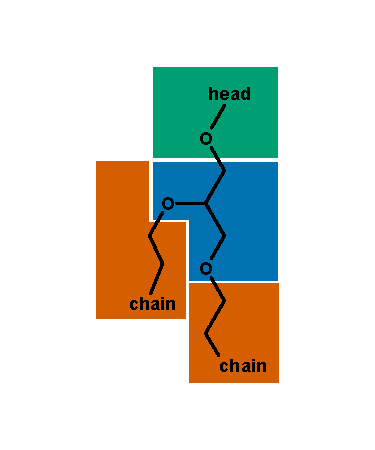
\includegraphics[width=1\linewidth]{figs_ch1/DEG}
        	\caption{DEG}
        \label{fig:DEG}
    \end{subfigure}
    \begin{subfigure}[b]{.3\linewidth}
    	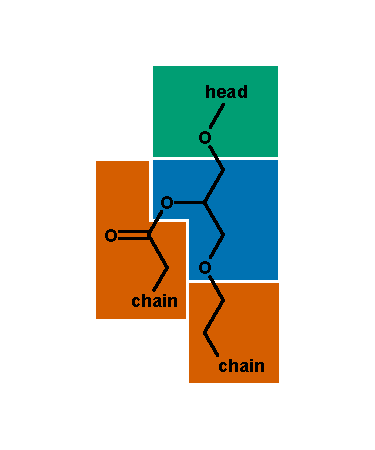
\includegraphics[width=1\linewidth]{figs_ch1/AEG}
    	\caption{AEG}
        \label{fig:AEG}
    \end{subfigure}
    \begin{subfigure}[b]{.3\linewidth}
        	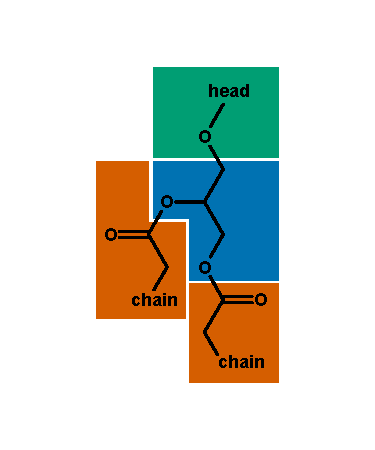
\includegraphics[width=\linewidth]{figs_ch1/DAG}
    	\caption{DAG}
        \label{fig:DAG}
    \end{subfigure}
    \begin{subfigure}[b]{.3\linewidth}
    	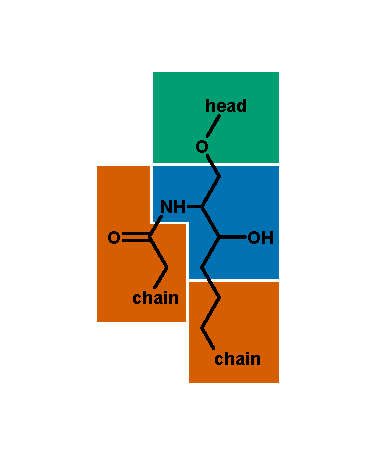
\includegraphics[width=\linewidth]{figs_ch1/CER}
    	\caption{CER}
        \label{fig:CER}
    \end{subfigure}
    \begin{subfigure}[b]{.3\linewidth}
    	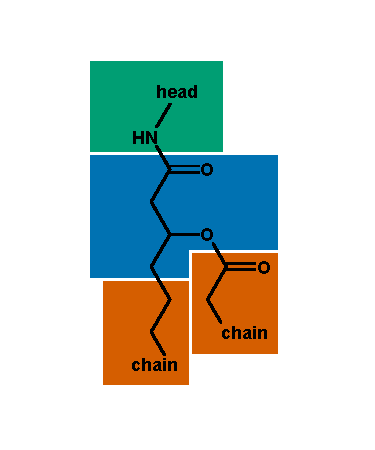
\includegraphics[width=\linewidth]{figs_ch1/FAHFAm}
    	\caption{FAHFAm}
        \label{fig:FAHFAm}
    \end{subfigure}
    \begin{subfigure}[b]{.3\linewidth}
        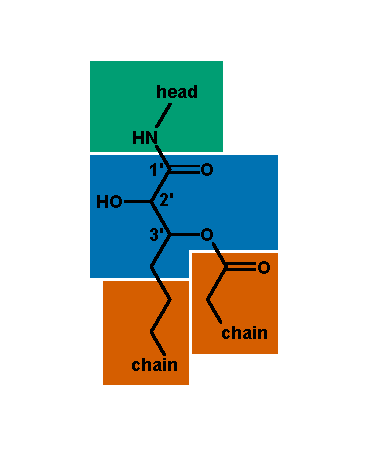
\includegraphics[width=\linewidth]{figs_ch1/FAHFAm-OH}
    	\caption{FAHFAm-OH*}
        \label{fig:FAHFAm-OH}
    \end{subfigure}
    \begin{subfigure}[b]{.6\linewidth}
        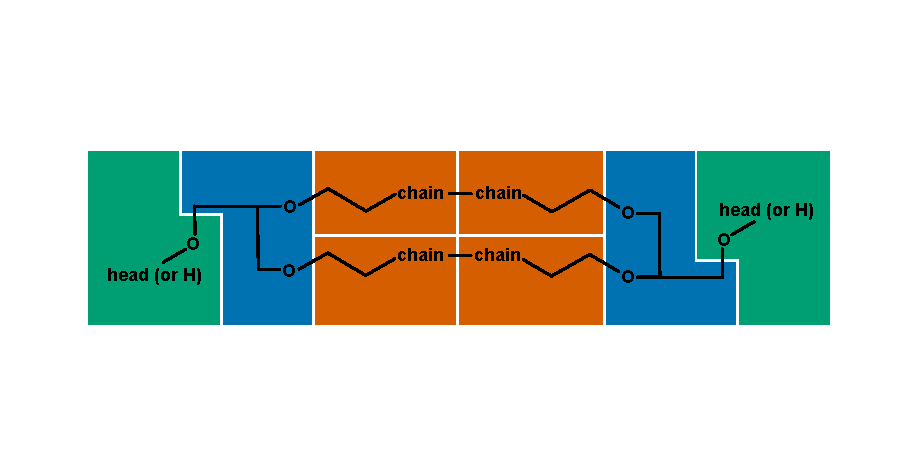
\includegraphics[width=\linewidth]{figs_ch1/GDGT}
    	\caption{GDGT}
        \label{fig:GDGT}
    \end{subfigure}
    \begin{subfigure}[b]{.3\linewidth}
    	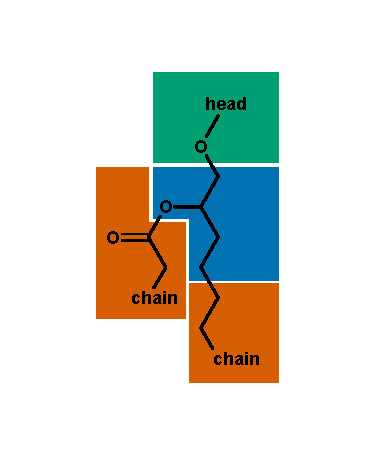
\includegraphics[width=\linewidth]{figs_ch1/alkanediol}
    	\caption{1,2-alkanediol}
        \label{fig:diol}
    \end{subfigure}
\end{figure}
\newpage
\begin{figure}[h]\ContinuedFloat

    \begin{subfigure}[b]{.3\linewidth}
    	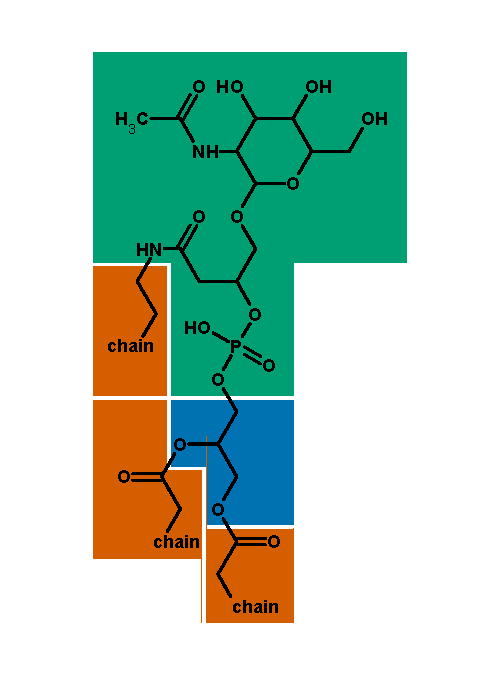
\includegraphics[width=\linewidth]{figs_ch1/NAcG-P-DAG}
    	\caption{NAcG-P-DAG}
        \label{fig:NAcG-P-DAG}
    \end{subfigure}
    \begin{subfigure}[b]{.3\linewidth}
    	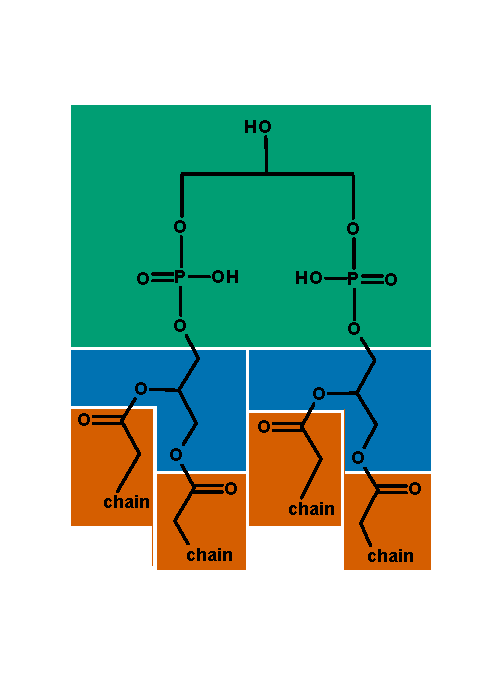
\includegraphics[width=\linewidth]{figs_ch1/DPG}
    	\caption{DPG}
        \label{fig:DPG}
    \end{subfigure}
    \begin{subfigure}[b]{.3\linewidth}
        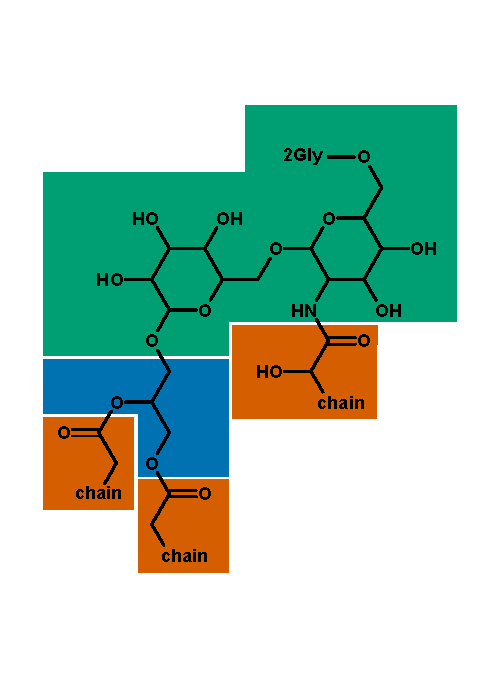
\includegraphics[width=\linewidth]{figs_ch1/2GNAcG-G-DAG}
    	\caption{2GNAcG-G-DAG**}
        \label{fig:2GNAcG-G-DAG}
    \end{subfigure}

    
\caption[Structural designations used for IPL headgroups, backbones, and alkyl chains]{Structural designations used for IPL headgroups, backbones, and alkyl chains, for the sake of calculating abundance-weighted average properties and chemical formulas. Abbreviations are defined in the text. Green boxes contain elemental abundances associated with headgroups, with only the headgroup-backbone connector group explicitly shown and the rest of the headgroup represented as `head'. Chemical formulae given in Table \ref{tab:IPL} represent elemental abundances of structures contained within the green box. Blue boxes contain backbone elemental abundances. Orange boxes designate elemental abundances belonging to alkyl chains. Only the chemical structure of the first two carbons of each alkyl chain are shown; with `chain' representing the rest. *In FAHFAm-OH, backbone-alkyl chain esterification may occur on either the 2' or 3' hydroxyl group \citep{diercks2015accumulation}. **Referred to as NAcG-DAG in \cite{schubotz2013spatial}}
\label{fig:IPLdivision}
\end{figure}
\doublespace
\clearpage
}


% % These components have been categorized into three major structural motifs; headgroups, backbones, and alkyl chains. Backbones linked to alkyl chains are referred to here as `tailgroups'. 

% % When considering differences in these motifs across lipid structures, it becomes important to define boundaries between these components for the sake of consistently comparing properties that depend on chemical formulas (such as Z\textsubscript{C} or alkyl chain length), particularly for IPLs without a `traditional' glycerol backbone, such as 1,2-alkanediols, CER-lipids, and FAHFAm-lipids (Figure \ref{fig:diol}, \subref{fig:CER}, and \subref{fig:FAHFAm}/\subref{fig:FAHFAm-OH}, respectively). Described below are the definitions applied to all observed IPL structures to designate chemical formulae of headgroup, backbone, and alkyl chains.

The portion of an IPL comprising a headgroup was structurally designated as one or more covalently-bonded polar moieties linked to one or more backbones, and is represented by structures contained within green boxes in Figure \ref{fig:IPLdivision}. In some cases, the headgroup itself may be directly linked to one or more alkyl chains, such as in the tentative structures shown in Figures \ref{fig:NAcG-P-DAG} and \ref{fig:2GNAcG-G-DAG}. To calculate consistent chemical formulae, headgroups include electronegative atoms linking them to backbones or chains, such as the oxygen atom that forms the glycosidic bond between backbone and sugar headgroup in a glycolipid. Furthermore, the chemical formulae of all headgroups are calculated for their neutrally-charged state, with the +1 charge imparted by quaternary ammonium functional of cationic lipids PC, TM-OL, TM-OL-OH, and TM-KL serving as the only exception because this charge is not the result of pH-dependent ionization.

Backbone structures are designated by blue boxes in Figure \ref{fig:IPLdivision}. In this study, IPL backbones were structurally designated according to three criteria chosen to promote consistency between observed IPL structures. First, the backbone must have a linear aliphatic chain of three carbons. Second, one carbon must be covalently bonded to an IPL headgroup. Third, the backbone must include two `connector' functional groups that serve to anchor alkyl chains. Various backbone-alkyl chain linkage types are shown in Figure \ref{fig:chain_comparison}, with backbone connector groups shown proximal to the R\textsubscript{1} group representing the rest of the backbone; -CH$_{2}$- for a carbon-carbon (C-C) link (\textit{e.g.} Figure \ref{fig:chain_comparison}a), -O- for an ether link (\textit{e.g.} Figure \ref{fig:chain_comparison}b, c, d, and e), -NH- for an amide link (\textit{e.g.} Figure \ref{fig:chain_comparison}f), or -O- for an ester link (\textit{e.g.} Figure \ref{fig:chain_comparison}g, h, i, and j). The decision to include connector groups in the structure of the backbone rather than in alkyl chains was made to maintain consistency when calculating nC in alkyl chains with C-C backbone-chain linkage relative to other chains. To demonstrate this point, consider the C-C linked alkyl chain in Figure \ref{fig:chain_comparison}a and the ether-linked alkyl chain in Figure \ref{fig:chain_comparison}b. Both are saturated and have approximately the same physical length. To ensure that both chains have the same value for nC, the `connector' groups proximal to the rest of the backbone, R\textsubscript{1}, must be categorized as part of the backbone structure.

\afterpage{
\singlespace
\begin{figure}
\centering
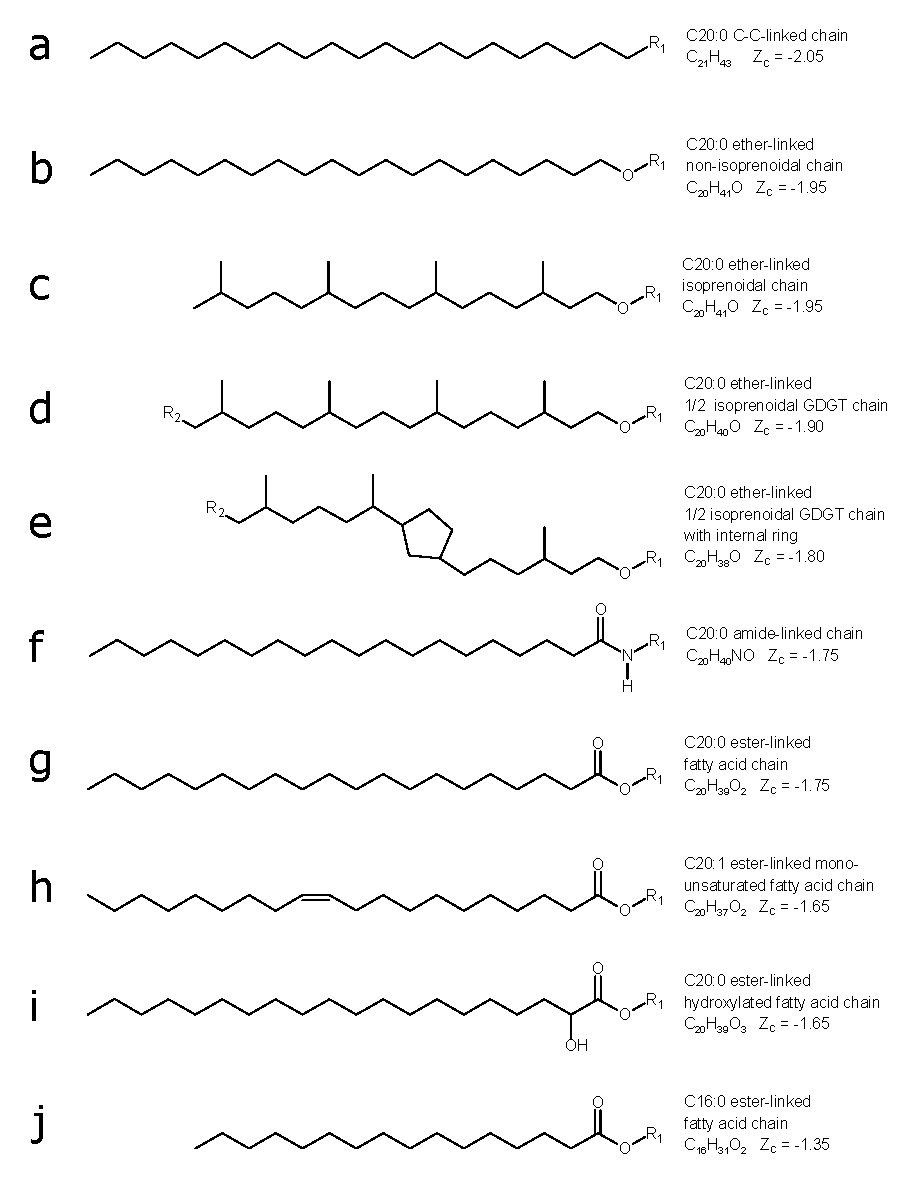
\includegraphics[width=.85\linewidth]{figs_ch1/chain_comparison}
\caption[Lipid alkyl chain modifications and backbone-chain linkage types organized by Z\textsubscript{C}]{Lipid alkyl chain modifications and backbone-chain linkage types organized by Z\textsubscript{C} from reduced (top) to oxidized (bottom). Example structures were chosen to permit comparison of Z\textsubscript{C} according to a various types of biochemical modifications: chain-backbone linkage type as C-C, ether, amide, or ester (a, b, f, g); non-branching and branching chains (b, c); bilayer- and monolayer-forming isoprenoidal chains (c, d); GDGT chains without and with an internal ring (d, e); saturated and unsaturated chains (g, h); non-hydroxylated and hydroxylated chains (g, i); and chains with a greater and lesser number of aliphatic carbons (g, j). R\textsubscript{1} represents the rest of the lipid backbone and R\textsubscript{2} indicates the second half of a monolayer-forming GDGT chain and is considered a separate chain when calculating average chain properties.}
\label{fig:chain_comparison}
\end{figure}
\doublespace
}

In addition to these two connector groups, the three-carbon backbone may include modifications such as hydroxylations or carbonyl groups. A single lipid may have more than one backbone, such as DPG or GDGT (Figure \ref{fig:DPG} and \ref{fig:GDGT}). 
% For `lyso'-IPLs with only one alkyl chain, the backbone is assigned one extra hydrogen atom to cap off the naked connector group.

Alkyl chains are aliphatic hydrocarbon chains linked to the IPL backbone or in some cases, directly to the headgroup. Their structural designation is indicated by orange boxes in Figure \ref{fig:IPLdivision}. To calculate consistent nC across all observed variations in IPL structure, each chain begins at the carbon directly after the backbone `connector' group and continues to the distal methyl group that caps the end of the chain. Alkyl chains of GDGTs provide the only exception to this, as they have two continuous monolayer-forming (membrane-spanning) isoprenoidal chains rather than two bilayer-forming chains common to non-GDGT IPLs. To calculate and compare chain properties across monolayer and bilayer-forming IPLs, each mole of GDGT is counted as having four moles of equal-length monolayer-forming chains (see Figure \ref{fig:GDGT}), with each chain covalently bonded to one other chain by a -CH\textsubscript{2}- group (\textit{e.g} Figure \ref{fig:chain_comparison}d or e).





\subsection{Calculation of average lipid properties and elemental composition}
Abundance-weighted properties of IPL headgroups, backbones, and chains were calculated for a sample using the equation

\begin{equation} \label{eq:avecomponent}
\Xi = \frac{\sum_{i} \Xi_{ipl,i} \cdot x_{i}}{\sum_{i} n_{component,i} \cdot x_{i}},
\end{equation}

\noindent where $\Xi$ indicates the average property of interest, $\Xi_{ipl,i}$ represents the property summed across all components in the $i^{th}$ IPL with a mole fraction of $x_{i}$ and $n_{component,i}$ number of the component of interest.

Abundance-weighted properties calculated in this way include nC, nUnsat, and the number of hydroxylations (nOH) per alkyl chain, the fraction of alkyl chains that form monolayers ($x_{monolayer}$), and the fraction backbone-alkyl chain linkage types with an ether ($x_{ether}$), ester ($x_{ester}$), amide ($x_{amide}$), or C-C ($x_{C-C}$) bond.

The abundance-weighted number of internal rings per GDGT (not per alkyl chain) in a sample was also calculated using Equation \ref{eq:avecomponent} by setting $x_{i}$ to the mole fraction of the $i^{th}$ GDGT (rather than the $i^{th}$ IPL), and setting $n_{component,i} \cdot x_{i}$ equal to 1, thereby producing a per-GDGT property rather than a per-chain property.

Average chemical formulae of IPL components were determined using known charge and elemental abundance of carbon, hydrogen, nitrogen, oxygen, phosphorus, and sulfur atoms in the chemical structures as $\Xi_{ipl,i}$ in Equation \ref{eq:avecomponent} and then solving for the weighted average of each. The average chemical formulae of full IPL structures was calculated using the charge and elemental abundance summed across the $i^{th}$ IPL while setting $n_{component,i} \cdot x_{i}$ equal to 1. Even when the structure of an IPL component is unclear (\textit{e.g}. the unidentified `223' headgroup observed in this study), its elemental composition is typically obtainable with accurate-mass spectrometry. This permits the inclusion of ambiguous structures when calculating average elemental abundances.

\subsection{Calculation of IPL Z\textsubscript{C}}
Abundance-weighted $Z_{C}$ for IPLs and their component parts were calculated using the abundance-weighted chemical formulae in the equation

\begin{equation} \label{eq:ZC}
{Z}_{C} = \frac{2o + 3n - 5p - 4s - h - Z}{c},
\end{equation}

\noindent where $Z$ stands for the net charge and $c$, $h$, $n$, $o$, $p$, and $s$ represent the number of atoms of carbon, hydrogen, nitrogen, oxygen, phosphorus, and sulfur in the chemical formula of interest. Hydrogen, oxygen, and nitrogen are assigned oxidation states of +1, -2, and -3. Sulfur within the sulfonic acid group of SQ-DAG is assigned an oxidation state of +4. Phosphorus is assigned an oxidation state of +5 to be consistent with that of phosphorus within the phosphate ion. Charge gained or lost by pH-dependent protonation or deprotonation, as is common in many lipid headgroups, does not require extra consideration, as this does not affect $Z_{C}$.

Equation \ref{eq:ZC} was also used to determine the Z\textsubscript{C} values of individual lipid structures, such as those reported in Figure \ref{fig:chain_comparison}.

\subsection{Simulation of analytical uncertainty} A Monte Carlo-style boostrap sensitivity analysis was performed in which manually-integrated IPL HPLC-MS peak areas were allowed to vary randomly by up to 30\% their original value, and analytical response factors applied to any headgroup-backbone combination listed in Table \ref{tab:IPL} were allowed to vary by up two orders of magnitude higher or lower over the course of 999 iterations. Abundance-weighted Z\textsubscript{C} for lipids and their components were re-calculated from abundance-weighted average chemical formulae after each iteration.


\section{Results}

\afterpage{

\singlespace
\begin{table}[htbp]
\begin{adjustbox}{width=\textwidth,keepaspectratio}
\begin{threeparttable}
  \caption{Selected geochemical and physical data from each sample site}
    % Table generated by Excel2LaTeX from sheet 'Geochemical and Physical Data'
% Table generated by Excel2LaTeX from sheet 'Geochemical and Physical Data'
\begin{tabular}{clccrcccc}
\toprule
      &       & \multicolumn{2}{c}{12T UTM coords.} & Dist\tnote{a} & Zone\tnote{b} & Temperature & pH    & Conductivity\tnote{c} \\
\cmidrule{3-4}Site  & Sample & easting & northing & (m)   &       & ($\degree$C) &       & ($\mu$S) \\
\midrule
Bison & BP1   & 510710 & 4935155 & 2.9   & C     & 89.0  & 7.23  & 1550 \\
Pool  & BP2   & 510715 & 4935156 & 8.2   & C     & 80.9  & 7.34  & 1568 \\
      & BP3   & 510718 & 4935157 & 11.1  & T     & 73.3  & 7.27  & 1540 \\
      & BP4   & 510719 & 4935159 & 13.4  & P     & 63.1  & 8.09  & - \\
      & BP5   & 510719 & 4935163 & 17.2  & P     & 40.5  & 8.25  & 1508 \\
      & BP6   & 510724 & 4935165 & 22.6  & P     & 29.0  & 9.01  & 1697 \\
      &       &       &       &       &       &       &       &  \\
Mound & MS1   & 511114 & 4934621 & 3.6   & C     & 91.0  & 8.81  & 1612 \\
Spring & MS2   & 511108 & 4934624 & 12.7  & C     & 77.3  & 8.65  & 1621 \\
      & MS3   & 511098 & 4934628 & 24.2  & P     & 64.8  & 9.08  & 1617 \\
      & MS4   & 511083 & 4934621 & 38.7  & P     & 53.0  & 9.22  & 1634 \\
      & MS5   & 511049 & 4934625 & 53    & P     & 35.1  & 9.53  & 1660 \\
      &       &       &       &       &       &       &       &  \\
Empress & EP1   & 0521589 & 4948280 & 2.2   & C     & 82.2  & 5.78  & 1824 \\
Pool  & EP2   & 0521585 & 4948280 & 6.2   & T     & 70.5  & 6.96  & 1832 \\
      & EP3   & 0521580 & 4948285 & 13.3  & T     & 60.7  & 7.63  & 1840 \\
      & EP4   & 0521560 & 4948293 & 34.8  & P     & 51.6  & 7.99  & 1860 \\
      & EP5   & 0521558 & 4948295 & 37.6  & P     & 38.1  & 8.42  & 1664 \\
      &       &       &       &       &       &       &       &  \\
Octopus & OS1   & 0516054 & 4931217 & 7.0   & C     & 85.4  & 7.29  & 1622 \\
Spring & OS2   & 0516016 & 4931212 & 38.3  & P     & 59.8  & 8.27  & 1581 \\
\bottomrule
\end{tabular}%

    \begin{tablenotes}
      \small
      \item[a] Distance from hot spring source.
      \item[b] Major metabolic regime representative of the microbial community at the sample site, interpreted visually in the field based on the presence or absence of photosynthetic pigments; C, strictly chemosynthetic; T, transition to phototrophy; P, photosynthetic.
      \item[c] Conductivity is normalized to 25\degree C using the formula Cond$_{T}/(1+\alpha(T-25))$, where Cond$_{T}$ is the conductivity measured at the temperature of the sample site and $\alpha$ is the temperature correction coefficient taken as 0.02 for freshwater.
    %   \item[d] Oxygen-18 isotope ratio relative to VSMOW.
    \end{tablenotes}
  \label{tab:geophysical}%
  \end{threeparttable}
  \end{adjustbox}
\end{table}%
\doublespace
\clearpage
}




\afterpage{
\singlespace
\begin{table}[htbp]
  \begin{adjustbox}{width=\textwidth,keepaspectratio}
  \begin{threeparttable}
  \caption[Concentrations of selected redox-sensitive dissolved chemical species]{Concentrations of selected redox-sensitive dissolved chemical species\textsuperscript{a}}


% Table generated by Excel2LaTeX from sheet 'Geochemical and Physical Data'
\begin{tabular}{clrrrrrr}
\toprule
      &       & \multicolumn{4}{c}{Oxidized}  & \multicolumn{2}{c}{Reduced} \\
\cmidrule(l{2pt}r{2pt}){3-6} \cmidrule(l{2pt}r{2pt}){7-8}      &       & \multicolumn{1}{c}{O\textsubscript{2}} & \multicolumn{1}{c}{NO\textsubscript{3}\textsuperscript{-}} & \multicolumn{1}{c}{NO\textsubscript{2}\textsuperscript{-}} & \multicolumn{1}{c}{$\sum$SO\textsubscript{4}\textsuperscript{2-}} & \multicolumn{1}{c}{$\sum$NH\textsubscript{4}\textsuperscript{+}} & \multicolumn{1}{c}{$\sum$HS\textsuperscript{-}} \\
Site  & Sample & \multicolumn{1}{c}{(mg l\textsuperscript{-1})} & \multicolumn{1}{c}{(mg l\textsuperscript{-1})} & \multicolumn{1}{c}{(mg l\textsuperscript{-1})} & \multicolumn{1}{c}{(mg l\textsuperscript{-1})} & \multicolumn{1}{c}{(mg l\textsuperscript{-1})} & \multicolumn{1}{c}{($\mu$g l\textsuperscript{-1})} \\
\midrule
Bison & BP1   & 0.2   & 0.01  & 0.02  & 13.11 & 0.07  & 230 \\
Pool  & BP2   & 0.7   & 0.01  & 0.04  & 15.43 & 0.06  & 220 \\
      & BP3   & 1.1   & 0.02  & 0.01  & 16.81 & 0.04  & bdl\tnote{b} \\
      & BP4   & 2.3   & 0.03  & 0.02  & 16.50 & 0.02  & 6 \\
      & BP5   & 5.7   & 0.004 & bdl   & 17.18 & 0.01  & 15 \\
      & BP6   & 3.3   & 0.07  & bdl   & 18.32 & 0.02  & 10 \\
      &       &       &       &       &       &       &  \\
Mound & MS1   & 0.4   & 0.01  & bdl   & 14.33 & 0.07  & 716 \\
Spring & MS2   & 2.2   & 0.01  & bdl   & 15.03 & 0.01  & 758 \\
      & MS3   & 1.4   & 0.04  & 0.02  & 16.99 & 0.03  & 236 \\
      & MS4   & 3.6   & 0.02  & 0.01  & 17.56 & 0.02  & 70 \\
      & MS5   & 6.9   & 0.06  & bdl   & 20.11 & bdl   & bdl \\
      &       &       &       &       &       &       &  \\
Empress & EP1   & 0.4   & 0.01  & 0.08  & 106.87 & 0.42  & 260 \\
Pool  & EP2   & 0.7   & -     & -     & -     & -     & 97 \\
      & EP3   & 1.2   & 0.01  & bdl   & 106.70 & 0.31  & 37 \\
      & EP4   & 1.3   & 0.03  & 0.03  & 111.70 & 0.39  & 31 \\
      & EP5   & 3.4   & 0.08  & 0.01  & 111.24 & 0.14  & 18 \\
      &       &       &       &       &       &       &  \\
Octopus & OS1   & 0.5   & 0.03  & 0.03  & 17.82 & 0.06  & 13 \\
Spring & OS2   & 3.3   & 0.03  & 0.02  & 18.76 & 0.02  & 12 \\
\bottomrule
\end{tabular}%


	\begin{tablenotes}
      \small
      \item[a] Note: Sulfide (HS\textsuperscript{-}), ammonium (NH\textsubscript{4}\textsuperscript{+}), and sulfate (SO\textsubscript{4}\textsuperscript{2-}) concentrations are summed for their respective pH-dependent protonated states.
      
      \item[b] bdl: below detection limit
      \normalsize
    \end{tablenotes}
  \label{tab:redox}%
  \end{threeparttable}
  \end{adjustbox}
\end{table}%
\doublespace
% to get nicer header midrules, replace \cmidrule{3-8} with
% \cmidrule(l{2pt}r{2pt}){3-6} \cmidrule(l{2pt}r{2pt}){7-8}
\clearpage
}

\afterpage{
\singlespace
\begin{figure}[h]
\centering
\includegraphics[width=1\linewidth]{"figs_ch1/scatterplot - hot spring redox"}
\caption[Total concentrations of redox-sensitive aqueous chemical species in samples from Bison Pool, Mound Spring, Empress Pool, and Octopus Spring]{Total concentrations of redox-sensitive aqueous chemical species in samples from Bison Pool (A), Mound Spring (B), Empress Pool (C) and Octopus Spring (D). Lines between points are meant to guide the eye between measurements only. A water sample was not collected for sulfate at Empress Pool site EP2 during the 2012 field season, indicated here by a dashed line between sulfate measurements for sites EP1 and EP3.}
\label{fig:redox}
\end{figure}
\doublespace
\clearpage
}


\subsection{Water chemistry and redox potential} Temperature, pH, and conductivity measurements corresponding to samples along the four studied hot spring outflow channels are shown in Table \ref{tab:geophysical}. As water flows from the source and cools, microbial communities in alkaline hot springs change spatially along the channel, with chemotrophs dominating the higher-temperature end and green/orange pigmented phototrophic cyanobacteria at the lower-temperature end. All four studied outflow channels show downstream changes in water chemistry as shown in Table \ref{tab:redox}, which in all cases are marked by an overall decrease in concentration of reduced inorganic dissolved species and an increase in concentration of oxidized inorganic solutes. It can be seen from Figure \ref{fig:redox} that concentrations of relatively reduced sulfide is more concentrated at the source and gradually give way to its oxidized counterpart sulfate, likely due to biological oxidation \citep{cox2011transition}. Previous research at Bison Pool and Mound Spring by \cite{loiacono2012evidence} demonstrated active expression of nitrogen-metabolizing genes by nitrifying microorganisms, likely explaining the downstream decrease of ammonia concentrations and concurrent increase in nitrite and nitrate concentrations reported in Table \ref{tab:redox}. The dissolved oxygen also exhibits an overall increase in concentration downstream, which can likely be attributed to flowing water mixing with the atmosphere, as well as input from oxygenic photosynthesis after the onset of cyanobacteria. Taken together, these geochemical data suggest that the redox potential of the water is generally more reduced at the hot spring source and gradually becomes more oxidized downstream.


\afterpage{
% \newgeometry{margin=1.5cm} % modify this if you need even more space
\begin{landscape}
\singlespace

\begin{table}
\centering
\normalsize
\begin{adjustbox}{width=600pt,keepaspectratio}
\begin{threeparttable}
  \caption{Weighted Z\textsubscript{C} and chemical formula of IPLs and their component parts}
 % to get nicer header midrules, replace \cmidrule{3-10} with
% \cmidrule(l{2pt}r{2pt}){3-6} \cmidrule(l{2pt}r{2pt}){7-10}


% Table generated by Excel2LaTeX from sheet 'ZC and chain formulae'
\begin{tabular}{lccccccccc}
\toprule
      &       & \multicolumn{4}{c}{Weighted Z\textsubscript{C}} & \multicolumn{4}{c}{Weighted chemical formula} \\
\cmidrule(l{2pt}r{2pt}){3-6} \cmidrule(l{2pt}r{2pt}){7-10}Site  & Sample & Full IPLs & Headgroups & Backbones & Alkyl chains & Full IPLs & Headgroups & Backbones & Alkyl chains \\
\midrule
Bison & BP1   & -1.56 & 0.15  & -0.34 & -1.92 & C\textsubscript{64.1}H\textsubscript{123.}N\textsubscript{2.15e-1}O\textsubscript{12.3}P\textsubscript{5.01e-1}S\textsubscript{1.27e-3}\textsuperscript{+8.04e-3} & C\textsubscript{5.61}H\textsubscript{11.0}N\textsubscript{1.46e-1}O\textsubscript{6.70}P\textsubscript{3.95e-1}S\textsubscript{9.55e-4}\textsuperscript{+6.07e-3} & C\textsubscript{3.02}H\textsubscript{5.05}N\textsubscript{1.71e-2}O\textsubscript{1.99} & C\textsubscript{19.8}H\textsubscript{38.5}O\textsubscript{2.85e-1} \\
Pool  & BP2   & -1.53 & 0.15  & -0.34 & -1.89 & C\textsubscript{56.9}H\textsubscript{109.}N\textsubscript{2.10e-1}O\textsubscript{12.3}P\textsubscript{6.07e-1}S\textsubscript{2.42e-3}\textsuperscript{+1.42e-2} & C\textsubscript{6.25}H\textsubscript{12.1}N\textsubscript{1.58e-1}O\textsubscript{7.62}P\textsubscript{5.34e-1}S\textsubscript{2.05e-3}\textsuperscript{+1.21e-2} & C\textsubscript{3.04}H\textsubscript{5.07}N\textsubscript{2.25e-2}O\textsubscript{1.99} & C\textsubscript{19.4}H\textsubscript{37.6}O\textsubscript{4.36e-1} \\
      & BP3   & -1.45 & 0.11  & -0.35 & -1.84 & C\textsubscript{48.0}H\textsubscript{91.5}N\textsubscript{1.48e-1}O\textsubscript{12.1}P\textsubscript{5.31e-1}S\textsubscript{8.32e-2}\textsuperscript{+4.61e-3} & C\textsubscript{6.71}H\textsubscript{12.9}N\textsubscript{1.03e-1}O\textsubscript{8.10}P\textsubscript{5.12e-1}S\textsubscript{7.95e-2}\textsuperscript{+4.40e-3} & C\textsubscript{3.06}H\textsubscript{5.12}N\textsubscript{3.89e-2}O\textsubscript{1.97} & C\textsubscript{17.9}H\textsubscript{34.5}O\textsubscript{7.54e-1} \\
      & BP4   & -1.46 & 0.13  & -0.35 & -1.88 & C\textsubscript{45.1}H\textsubscript{86.8}N\textsubscript{8.39e-2}O\textsubscript{12.1}P\textsubscript{6.25e-1}S\textsubscript{5.38e-2}\textsuperscript{+8.07e-3} & C\textsubscript{7.22}H\textsubscript{13.7}N\textsubscript{5.44e-2}O\textsubscript{8.90}P\textsubscript{6.23e-1}S\textsubscript{5.36e-2}\textsuperscript{+8.04e-3} & C\textsubscript{3.04}H\textsubscript{5.09}N\textsubscript{2.91e-2}O\textsubscript{1.97} & C\textsubscript{17.3}H\textsubscript{33.7}O\textsubscript{5.67e-1} \\
      & BP5   & -1.38 & 0.04  & -0.32 & -1.80 & C\textsubscript{44.6}H\textsubscript{83.7}N\textsubscript{3.32e-1}O\textsubscript{11.4}P\textsubscript{2.17e-1}S\textsubscript{1.21e-1}\textsuperscript{+1.24e-1} & C\textsubscript{7.82}H\textsubscript{14.6}N\textsubscript{3.26e-1}O\textsubscript{7.69}P\textsubscript{2.17e-1}S\textsubscript{1.21e-1}\textsuperscript{+1.24e-1} & C\textsubscript{3.11}H\textsubscript{5.02}N\textsubscript{5.65e-3}O\textsubscript{2.01} & C\textsubscript{16.8}H\textsubscript{32.0}O\textsubscript{8.49e-1} \\
      & BP6   & -1.36 & 0.02  & -0.33 & -1.73 & C\textsubscript{43.5}H\textsubscript{80.4}N\textsubscript{2.70e-1}O\textsubscript{11.6}P\textsubscript{4.64e-1}S\textsubscript{1.18e-1}\textsuperscript{+8.39e-2} & C\textsubscript{6.67}H\textsubscript{13.1}N\textsubscript{2.63e-1}O\textsubscript{7.57}P\textsubscript{4.63e-1}S\textsubscript{1.18e-1}\textsuperscript{+8.37e-2} & C\textsubscript{3.04}H\textsubscript{5.02}N\textsubscript{6.73e-3}O\textsubscript{2.00} & C\textsubscript{16.7}H\textsubscript{30.8}O\textsubscript{9.75e-1} \\
      &       &       &       &       &       &       &       &       &  \\
Mound & MS1   & -1.68 & 0.32  & -0.33 & -1.94 & C\textsubscript{92.2}H\textsubscript{177.}N\textsubscript{4.49e-4}O\textsubscript{11.2}P\textsubscript{2.43e-4}\textsuperscript{+7.34e-6} & C\textsubscript{3.14}H\textsubscript{6.23}N\textsubscript{1.29e-4}O\textsubscript{3.61}P\textsubscript{1.22e-4}\textsuperscript{+3.67e-6} & C\textsubscript{3.00}H\textsubscript{5.00}N\textsubscript{9.56e-5}O\textsubscript{2.00} & C\textsubscript{20.0}H\textsubscript{38.8}O\textsubscript{3.52e-4} \\
Spring & MS2   & -1.61 & 0.18  & -0.38 & -1.93 & C\textsubscript{68.7}H\textsubscript{133.}N\textsubscript{2.22e-1}O\textsubscript{12.0}P\textsubscript{3.77e-1}S\textsubscript{2.10e-2}\textsuperscript{+4.40e-3} & C\textsubscript{5.12}H\textsubscript{9.87}N\textsubscript{7.51e-2}O\textsubscript{5.98}P\textsubscript{2.65e-1}S\textsubscript{1.46e-2}\textsuperscript{+3.06e-3} & C\textsubscript{3.09}H\textsubscript{5.24}N\textsubscript{8.02e-2}O\textsubscript{1.92} & C\textsubscript{19.6}H\textsubscript{38.2}O\textsubscript{2.12e-1} \\
      & MS3   & -1.52 & 0.14  & -0.35 & -1.92 & C\textsubscript{49.9}H\textsubscript{96.5}N\textsubscript{4.98e-2}O\textsubscript{11.9}P\textsubscript{6.47e-1}S\textsubscript{2.03e-2}\textsuperscript{+1.27e-3} & C\textsubscript{6.57}H\textsubscript{12.6}N\textsubscript{1.72e-2}O\textsubscript{8.26}P\textsubscript{5.94e-1}S\textsubscript{1.86e-2}\textsuperscript{+1.17e-3} & C\textsubscript{3.03}H\textsubscript{5.09}N\textsubscript{2.84e-2}O\textsubscript{1.97} & C\textsubscript{18.0}H\textsubscript{35.3}O\textsubscript{3.30e-1} \\
      & MS4   & -1.43 & 0.06  & -0.34 & -1.82 & C\textsubscript{47.2}H\textsubscript{89.6}N\textsubscript{2.07e-1}O\textsubscript{12.1}P\textsubscript{4.93e-1}S\textsubscript{5.34e-2}\textsuperscript{+5.00e-2} & C\textsubscript{7.20}H\textsubscript{13.8}N\textsubscript{1.91e-1}O\textsubscript{8.12}P\textsubscript{4.78e-1}S\textsubscript{5.18e-2}\textsuperscript{+4.85e-2} & C\textsubscript{3.03}H\textsubscript{5.03}N\textsubscript{9.59e-3}O\textsubscript{1.99} & C\textsubscript{17.4}H\textsubscript{33.3}O\textsubscript{7.89e-1} \\
      & MS5   & -1.33 & -0.07 & -0.34 & -1.71 & C\textsubscript{46.6}H\textsubscript{85.5}N\textsubscript{2.60e-1}O\textsubscript{12.5}P\textsubscript{3.65e-1}S\textsubscript{1.25e-1}\textsuperscript{+1.69e-1} & C\textsubscript{8.29}H\textsubscript{15.9}N\textsubscript{2.51e-1}O\textsubscript{8.36}P\textsubscript{3.62e-1}S\textsubscript{1.24e-1}\textsuperscript{+1.68e-1} & C\textsubscript{3.04}H\textsubscript{5.02}N\textsubscript{7.05e-3}O\textsubscript{1.99} & C\textsubscript{16.8}H\textsubscript{30.7}O\textsubscript{9.51e-1} \\
      &       &       &       &       &       &       &       &       &  \\
Empress & EP1   & -1.60 & 0.22  & -0.33 & -1.96 & C\textsubscript{85.0}H\textsubscript{164.}N\textsubscript{1.17e-1}O\textsubscript{13.8}P\textsubscript{4.38e-2}\textsuperscript{+2.05e-4} & C\textsubscript{5.66}H\textsubscript{10.4}N\textsubscript{6.51e-2}O\textsubscript{5.79}P\textsubscript{2.97e-2}\textsuperscript{+1.16e-4} & C\textsubscript{3.00}H\textsubscript{5.01}N\textsubscript{2.23e-3}O\textsubscript{2.00} & C\textsubscript{19.8}H\textsubscript{38.8}O\textsubscript{1.61e-2} \\
Pool  & EP2   & -1.54 & 0.15  & -0.36 & -1.92 & C\textsubscript{62.0}H\textsubscript{119.}N\textsubscript{1.87e-1}O\textsubscript{12.5}P\textsubscript{4.18e-1}S\textsubscript{1.16e-2}\textsuperscript{+8.26e-3} & C\textsubscript{6.22}H\textsubscript{11.8}N\textsubscript{8.79e-2}O\textsubscript{7.06}P\textsubscript{3.28e-1}S\textsubscript{8.81e-3}\textsuperscript{+6.30e-3} & C\textsubscript{3.07}H\textsubscript{5.17}N\textsubscript{5.52e-2}O\textsubscript{1.95} & C\textsubscript{18.9}H\textsubscript{36.8}O\textsubscript{2.61e-1} \\
      & EP3   & -1.54 & 0.15  & -0.34 & -1.90 & C\textsubscript{67.9}H\textsubscript{130.}N\textsubscript{1.06e-1}O\textsubscript{13.4}P\textsubscript{3.20e-1}S\textsubscript{3.36e-2}\textsuperscript{+1.15e-2} & C\textsubscript{6.11}H\textsubscript{11.5}N\textsubscript{5.37e-2}O\textsubscript{6.74}P\textsubscript{2.32e-1}S\textsubscript{2.34e-2}\textsuperscript{+7.98e-3} & C\textsubscript{3.03}H\textsubscript{5.06}N\textsubscript{2.05e-2}O\textsubscript{1.98} & C\textsubscript{19.1}H\textsubscript{36.9}O\textsubscript{2.95e-1} \\
      & EP4   & -1.44 & 0.08  & -0.33 & -1.83 & C\textsubscript{51.6}H\textsubscript{97.2}N\textsubscript{2.52e-1}O\textsubscript{11.7}P\textsubscript{1.99e-1}S\textsubscript{1.13e-1}\textsuperscript{+8.90e-2} & C\textsubscript{6.88}H\textsubscript{12.9}N\textsubscript{2.11e-1}O\textsubscript{7.00}P\textsubscript{1.78e-1}S\textsubscript{9.96e-2}\textsuperscript{+7.87e-2} & C\textsubscript{3.07}H\textsubscript{5.04}N\textsubscript{1.18e-2}O\textsubscript{2.00} & C\textsubscript{17.8}H\textsubscript{33.9}O\textsubscript{6.78e-1} \\
      & EP5   & -1.37 & -0.01 & -0.31 & -1.77 & C\textsubscript{48.1}H\textsubscript{89.0}N\textsubscript{3.69e-1}O\textsubscript{11.6}P\textsubscript{8.99e-2}S\textsubscript{1.79e-1}\textsuperscript{+1.57e-1} & C\textsubscript{7.78}H\textsubscript{14.6}N\textsubscript{3.44e-1}O\textsubscript{7.23}P\textsubscript{8.53e-2}S\textsubscript{1.68e-1}\textsuperscript{+1.47e-1} & C\textsubscript{3.11}H\textsubscript{5.00}N\textsubscript{1.48e-3}O\textsubscript{2.01} & C\textsubscript{17.1}H\textsubscript{31.9}O\textsubscript{8.12e-1} \\
      &       &       &       &       &       &       &       &       &  \\
Octopus & OS1   & -1.56 & 0.13  & -0.34 & -1.95 & C\textsubscript{64.4}H\textsubscript{125.}N\textsubscript{9.12e-2}O\textsubscript{13.7}P\textsubscript{5.91e-1}S\textsubscript{2.83e-3}\textsuperscript{+1.45e-3} & C\textsubscript{6.97}H\textsubscript{13.3}N\textsubscript{8.14e-2}O\textsubscript{8.32}P\textsubscript{5.36e-1}S\textsubscript{2.23e-3}\textsuperscript{+1.15e-3} & C\textsubscript{3.01}H\textsubscript{5.02}N\textsubscript{5.92e-3}O\textsubscript{1.99} & C\textsubscript{20.4}H\textsubscript{40.3}O\textsubscript{2.63e-1} \\
Spring & OS2   & -1.48 & 0.12  & -0.34 & -1.89 & C\textsubscript{45.2}H\textsubscript{87.3}N\textsubscript{1.01e-1}O\textsubscript{11.9}P\textsubscript{6.79e-1}S\textsubscript{4.19e-2}\textsuperscript{+1.93e-2} & C\textsubscript{6.91}H\textsubscript{13.3}N\textsubscript{8.39e-2}O\textsubscript{8.72}P\textsubscript{6.78e-1}S\textsubscript{4.18e-2}\textsuperscript{+1.93e-2} & C\textsubscript{3.03}H\textsubscript{5.05}N\textsubscript{1.69e-2}O\textsubscript{1.99} & C\textsubscript{17.5}H\textsubscript{34.2}O\textsubscript{5.73e-1} \\
\bottomrule
\end{tabular}%


\begin{tablenotes}

\item
% \item [a] Full IPL structure.
% \item [b] Headgroup structure only.
% \item [c] Backbone structure only.
% \item [d] Alkyl chain structure only.

\end{tablenotes}

  \label{tab:IPL_ZC}
  \end{threeparttable}
  \end{adjustbox}
\end{table}

\end{landscape}
\doublespace
\clearpage
}




\afterpage{
\singlespace
\begin{figure}[h]
\centering
    \begin{subfigure}[b]{0.81\linewidth}
        	\includegraphics[width=1\linewidth]{"figs_ch1/scatterplot - weighted ZC of IPL components vs temp and logO2"}
    \end{subfigure}
    \begin{subfigure}[b]{0.18\linewidth}
        	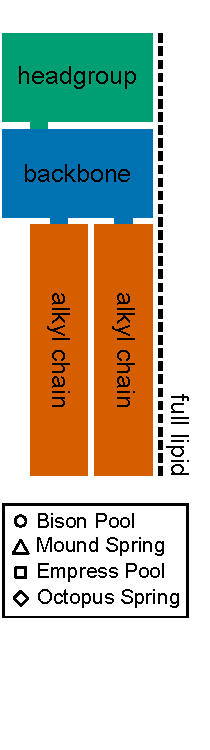
\includegraphics[width=1\linewidth]{figs_ch1/BasicLipidSchematic.pdf}
    \end{subfigure}
\caption[Abundance-weighted Z\textsubscript{C} of IPLs and their component parts]{Abundance-weighted Z\textsubscript{C} of headgroups (green), backbones (blue), alkyl chains (orange) and full (black) thermophile IPLs sampled along the outflow channels of four Yellowstone hot springs with respect to temperature (left) and log molality of dissolved O\textsubscript{2} (right). Observed values of weighted Z\textsubscript{C} of extracted lipids and their components are indicated by points. Bars and best-fit lines show the standard deviation and linear regression of 999 weighted Z\textsubscript{C} resulting from the bootstrap sensitivity analysis. Shaded areas represent 95\% intervals for the prediction of future bootstrap Z\textsubscript{C} values.}
\label{fig:weighted_ZC}
\end{figure}
\doublespace
\clearpage
}

\subsection{Z\textsubscript{C} of IPLs and their component parts}

The abundance-weighted chemical formulae and Z\textsubscript{C} calculated for thermophilic microbial IPLs and their headgroups, backbones, and alkyl chains are reported in Table \ref{tab:IPL_ZC} for samples collected from Bison Pool, Mound Spring, Empress Pool, and Octopus Spring. As shown in Figure \ref{fig:weighted_ZC}, decreasing temperature and increasingly oxidized conditions coincide with near-linear changes in the weighted Z\textsubscript{C} of IPLs and their components. Carbon was most reduced in IPLs sampled closest to the spring sources (Z\textsubscript{C} between -1.68 and -1.56) where temperatures were highest (82.2 to 91.0$^\circ$C) and concentrations of oxidized inorganic species (nitrate, sulfate, and oxygen) were lowest. In progressively downstream samples, carbon in IPLs became more oxidized, with weighted Z\textsubscript{C} between -1.36 and -1.33 for samples in the 29.0 to 38.1$^\circ$C temperature range where measured concentrations of sulfate, nitrate, and oxygen tended to be greatest. This trend persists even after simulating potential sources of analytical error, as shown in Figure \ref{fig:weighted_ZC} by the black bars above and below the `canon' observations of abundance-weighted Z\textsubscript{C}, which indicate the standard deviation of weighted Z\textsubscript{C} resulting from 999 iterations of the bootstrap sensitivity analysis. The standard deviations of IPL weighted Z\textsubscript{C} show little overlap between upstream and downstream samples after random variation of up to 30\% for integrated HPLC-MS peak areas and up to two orders of magnitude for response factors.

Alkyl chains tend to have weighted Z\textsubscript{C} approximately 0.3-0.4 more negative than those of the full structure regardless of sample. Compared to headgroups and backbones, the weighted Z\textsubscript{C} of alkyl chains were closest to that of the full structure, implicating this component as the primary contributor to full IPL Z\textsubscript{C} and observed trends with temperature and redox. This agrees with the observation that most carbon in IPLs belongs to the alkyl chains. Since alkyl chains have a high H/C ratio to facilitate their hydrophobicity, the weighted ZC of full IPLs and their chains are significantly more negative than those of backbones and headgroups, which have a higher ratio of electronegative atoms (e.g. oxygen, nitrogen) to carbon as a consequence of their relative hydrophilicity. As shown by in Figure \ref{fig:weighted_ZC}, trends in alkyl chain Z\textsubscript{C} appear to be more resilient to simulated sources of analytical uncertainty than the full structure based on sample standard deviations and the narrow 95\% prediction interval generated by the boostrap sensitivity analysis. The width of the prediction interval for future bootstrap results does not overlap between the highest temperature and lowest temperature, which the authors interpret as further evidence observed trends in alkyl chains are not artifacts of the analytical method used to quantify lipid abundance.

The weighted Z\textsubscript{C} of IPL backbones did not change significantly with temperature or redox, as most observed backbones were comprised of glycerol regardless of sample. According to the IPL component division scheme used in this study, an IPL glycerol backbone has a chemical formula of C\textsubscript{3}H\textsubscript{5}O\textsubscript{2}, corresponding to a Z\textsubscript{C} of $-0.\overline{3}$. This is close to the abundance-weighted value in every sample, with little variation.

Carbon in headgroups was significantly more oxidized than any other component, with weighted Z\textsubscript{C} ranging between -0.01 to 0.32 across samples. Glycolipid headgroups 1G (Z\textsubscript{C} = $0.1\overline{6}$) and 2G (Z\textsubscript{C} = $0.08\overline{3}$) were among the most abundant headgroups observed in all four springs regardless of temperature or redox, though they were most abundant, along with the glycolipid SQ (Z\textsubscript{C} = $0.1\overline{6}$) in samples where photosynthetic microorganisms are visually apparent. This agrees with observations that 1G, 2G, and SQ glycolipids are abundant in cyanobacterial \citep{wada2009lipids} and algal \citep{guschina2006lipids} photosynthetic membranes.

Phosphate-bearing phospholipids and glycophospholipids, especially lipids with PI headgroups, were more abundant downstream than upstream, though the incorporation of phosphate into the glycolipid headgroups had little to no affect on abundance-weighted headgroup Z\textsubscript{C}, as there is no difference in Z\textsubscript{C} between analogous nonphosphorylated and phosphorylated headgroups (\textit{e.g.} no difference in Z\textsubscript{C} between 1G-P and 1G, or between 2G-P and 2G, \textit{etc.}). The greatest abundance of lipids with an APT phospholipid headgroup (Z\textsubscript{C} = -0.2) was observed in `pink streamer' thermophile communities sampled from the upstream chemosynthetic zones of Bison Pool and Octopus Spring, which agrees with previous reports of this lipid is common in streamers dominated by \textit{Aquificales} bacteria \citep{Sturt_Intact_2004, schubotz2013spatial}. However, after applying response factors, the abundance APT was scarce relative to other headgroups, even in streamer samples.

% % Sollich paper: "acyl chains of BL, another well-known component of photosynthetic membranes (Dembitsky, 1996; Kato et al., 1996)"

% % Sollich paper: PC and CL (DPG) are common in mitochondria, and euk membranes tend to be rich with ceramides and sphingomyelin. We don't see much of that at cooler sites, though we tend to see more 'uncommon' phosphate-based PE, PG, PI, therefore we guess that bacteria, and not euk, dominate at those sites.

Intriguingly, weighted Z\textsubscript{C} of IPL headgroups became progressively negative with decreasing temperature or increasingly oxidized conditions, which is the reverse of trends observed alkyl chains and full IPLs. One reason for this stems from the way abundance-weighted Z\textsubscript{C} is calculated for GDGT headgroups. Because of the monolayer-forming properties of GDGTs, one mole of GDGT will have two moles of headgroup. As an example, consider that 1G-GDGT actually has two headgroups; the first is a glycosyl moiety linked to glycerol one one side of the GDGT, and the second is a hydroxyl (-OH) group terminating the glycerol on the other side of the GDGT. Summing the elemental abundances of 1G (C\textsubscript{6}H\textsubscript{11}O\textsubscript{6}) and -OH results in a total of C\textsubscript{6}H\textsubscript{12}O\textsubscript{7} for both headgroups of 1G-GDGT, or C\textsubscript{3}H\textsubscript{6}O\textsubscript{3.5} per headgroup. Accounting for this extra -OH means that the carbon in the headgroups of 1G-GDGT (Z\textsubscript{C} = $0.\overline{3}$) is considerably more oxidized than carbon in 1G headgroups of non-GDGTs (Z\textsubscript{C} = $0.1\overline{6}$). While 1G served here as an example, this extra oxygen and hydrogen atom must be accounted for in \textit{all} GDGTs, resulting in more oxidized headgroup carbon in high-temperature GDGT-dominated samples than one might expect based on headgroup identity. Another factor contributing to observed trends in the weighted Z\textsubscript{C} of IPL headgroups is a greater abundance of multi-methylated headgroups downstream, such as PC (Z\textsubscript{C} = $-1.4$), TM-OL (Z\textsubscript{C} = $-0.875$), TM-lysine (Z\textsubscript{C} = $-1.00$). Each methylation increases the H/C ratio of a headgroup substantially, resulting in more reduced carbon.

Regardless, trends in the weighted Z\textsubscript{C} of IPL headgroups appear to be substantially influenced by the sources of analytical uncertainty simulated by the bootstrap sensitivity analysis, especially for the low temperature downstream samples. As shown in Figure \ref{fig:weighted_ZC}, weighted Z\textsubscript{C} of headgroups in most samples show overlap in the vertical bars representing the simulated standard deviation. Furthermore, the 95\% prediction interval for future bootstrap calculations is widest for headgroups, with significant overlap between prediction range at the samples furthest upstream and downstream. This calls into question the significance of the apparent headgroup ZC trends with temperature and redox, as these trends may be an artifact of the analytical method used to quantify lipids.



\afterpage{
\begin{landscape}
\singlespace

\begin{table}
\centering
\normalsize
\begin{adjustbox}{width=600pt,keepaspectratio}
\begin{threeparttable}
  \caption{Summary of abundance-weighted alkyl chain properties}
  

% Table generated by Excel2LaTeX from sheet 'Chain properties'
\begin{tabular}{lccccllcccc}
\toprule
      &       &       &       &       & \multicolumn{5}{c}{Mole fraction alkyl chain or linkage type} & Rings per \\
\cmidrule{6-10}Site  & Sample & nC    & nUnsat & nOH   & \multicolumn{1}{c}{$x_{monolayer}$} & \multicolumn{1}{c}{$x_{ether}$} & $x_{ester}$ & $x_{amide}$ & $x_{C-C}$ & GDGT \\
\midrule
Bison & BP1   & 19.80 & 3.12$\cdot 10$\textsuperscript{-1} & 2.10$\cdot 10$\textsuperscript{-3} & 4.90$\cdot 10$\textsuperscript{-1} & 7.03$\cdot 10$\textsuperscript{-1} & 2.75$\cdot 10$\textsuperscript{-1} & 1.11$\cdot 10$\textsuperscript{-2} & 1.09$\cdot 10$\textsuperscript{-2} & 1.8 \\
Pool  & BP2   & 19.39 & 3.62$\cdot 10$\textsuperscript{-1} & 5.27$\cdot 10$\textsuperscript{-3} & 3.00$\cdot 10$\textsuperscript{-1} & 5.46$\cdot 10$\textsuperscript{-1} & 4.18$\cdot 10$\textsuperscript{-1} & 1.64$\cdot 10$\textsuperscript{-2} & 1.92$\cdot 10$\textsuperscript{-2} & 2.2 \\
      & BP3   & 17.94 & 3.34$\cdot 10$\textsuperscript{-1} & 5.91$\cdot 10$\textsuperscript{-3} & 8.81$\cdot 10$\textsuperscript{-2} & 2.17$\cdot 10$\textsuperscript{-1} & 7.32$\cdot 10$\textsuperscript{-1} & 2.37$\cdot 10$\textsuperscript{-2} & 2.79$\cdot 10$\textsuperscript{-2} & 2.8 \\
      & BP4   & 17.28 & 3.46$\cdot 10$\textsuperscript{-1} & 4.70$\cdot 10$\textsuperscript{-3} & 7.16$\cdot 10$\textsuperscript{-3} & 4.14$\cdot 10$\textsuperscript{-1} & 5.52$\cdot 10$\textsuperscript{-1} & 1.51$\cdot 10$\textsuperscript{-2} & 1.88$\cdot 10$\textsuperscript{-2} & 3.1 \\
      & BP5   & 16.82 & 4.91$\cdot 10$\textsuperscript{-1} & 2.93$\cdot 10$\textsuperscript{-4} & 7.20$\cdot 10$\textsuperscript{-4} & 9.80$\cdot 10$\textsuperscript{-2} & 8.46$\cdot 10$\textsuperscript{-1} & 2.83$\cdot 10$\textsuperscript{-3} & 5.33$\cdot 10$\textsuperscript{-2} & 3.2 \\
      & BP6   & 16.68 & 8.10$\cdot 10$\textsuperscript{-1} & 3.03$\cdot 10$\textsuperscript{-3} & 2.94$\cdot 10$\textsuperscript{-3} & 3.28$\cdot 10$\textsuperscript{-3} & 9.72$\cdot 10$\textsuperscript{-1} & 3.36$\cdot 10$\textsuperscript{-3} & 2.15$\cdot 10$\textsuperscript{-2} & 3.3 \\
      &       &       &       &       &       &       &       &       &       &  \\
Mound & MS1   & 20.00 & 2.72$\cdot 10$\textsuperscript{-4} & -     & 9.99$\cdot 10$\textsuperscript{-1} & \multicolumn{1}{c}{$<$ 1.00} & 3.04$\cdot 10$\textsuperscript{-4} & 4.78$\cdot 10$\textsuperscript{-5} & 4.96$\cdot 10$\textsuperscript{-5} & 2.5 \\
Spring & MS2   & 19.60 & 1.94$\cdot 10$\textsuperscript{-1} & 7.79$\cdot 10$\textsuperscript{-4} & 6.07$\cdot 10$\textsuperscript{-1} & 7.39$\cdot 10$\textsuperscript{-1} & 1.71$\cdot 10$\textsuperscript{-1} & 4.74$\cdot 10$\textsuperscript{-2} & 4.33$\cdot 10$\textsuperscript{-2} & 2.0 \\
      & MS3   & 18.01 & 3.53$\cdot 10$\textsuperscript{-1} & 7.06$\cdot 10$\textsuperscript{-4} & 1.64$\cdot 10$\textsuperscript{-1} & 6.54$\cdot 10$\textsuperscript{-1} & 3.15$\cdot 10$\textsuperscript{-1} & 1.55$\cdot 10$\textsuperscript{-2} & 1.50$\cdot 10$\textsuperscript{-2} & 2.8 \\
      & MS4   & 17.38 & 3.88$\cdot 10$\textsuperscript{-1} & 1.48$\cdot 10$\textsuperscript{-4} & 5.85$\cdot 10$\textsuperscript{-2} & 1.94$\cdot 10$\textsuperscript{-1} & 7.84$\cdot 10$\textsuperscript{-1} & 5.10$\cdot 10$\textsuperscript{-3} & 1.69$\cdot 10$\textsuperscript{-2} & 2.9 \\
      & MS5   & 16.78 & 9.65$\cdot 10$\textsuperscript{-1} & 3.39$\cdot 10$\textsuperscript{-5} & 1.09$\cdot 10$\textsuperscript{-2} & 2.68$\cdot 10$\textsuperscript{-2} & 9.47$\cdot 10$\textsuperscript{-1} & 3.52$\cdot 10$\textsuperscript{-3} & 2.23$\cdot 10$\textsuperscript{-2} & 3.5 \\
      &       &       &       &       &       &       &       &       &       &  \\
Empress & EP1   & 19.83 & 1.51$\cdot 10$\textsuperscript{-2} & 2.35$\cdot 10$\textsuperscript{-4} & 8.63$\cdot 10$\textsuperscript{-1} & 9.83$\cdot 10$\textsuperscript{-1} & 1.47$\cdot 10$\textsuperscript{-2} & 1.11$\cdot 10$\textsuperscript{-3} & 1.13$\cdot 10$\textsuperscript{-3} & 2.1 \\
Pool  & EP2   & 18.91 & 2.24$\cdot 10$\textsuperscript{-1} & 1.34$\cdot 10$\textsuperscript{-2} & 4.71$\cdot 10$\textsuperscript{-1} & 7.06$\cdot 10$\textsuperscript{-1} & 2.30$\cdot 10$\textsuperscript{-1} & 3.15$\cdot 10$\textsuperscript{-2} & 3.25$\cdot 10$\textsuperscript{-2} & 2.5 \\
      & EP3   & 19.06 & 1.37$\cdot 10$\textsuperscript{-1} & 6.14$\cdot 10$\textsuperscript{-3} & 6.06$\cdot 10$\textsuperscript{-1} & 6.88$\cdot 10$\textsuperscript{-1} & 2.85$\cdot 10$\textsuperscript{-1} & 1.07$\cdot 10$\textsuperscript{-2} & 1.65$\cdot 10$\textsuperscript{-2} & 2.5 \\
      & EP4   & 17.78 & 3.97$\cdot 10$\textsuperscript{-1} & 3.88$\cdot 10$\textsuperscript{-3} & 2.31$\cdot 10$\textsuperscript{-1} & 2.84$\cdot 10$\textsuperscript{-1} & 6.72$\cdot 10$\textsuperscript{-1} & 5.91$\cdot 10$\textsuperscript{-3} & 3.75$\cdot 10$\textsuperscript{-2} & 2.5 \\
      & EP5   & 17.08 & 6.87$\cdot 10$\textsuperscript{-1} & 4.47$\cdot 10$\textsuperscript{-4} & 1.26$\cdot 10$\textsuperscript{-1} & 1.32$\cdot 10$\textsuperscript{-1} & 8.11$\cdot 10$\textsuperscript{-1} & 7.42$\cdot 10$\textsuperscript{-4} & 5.62$\cdot 10$\textsuperscript{-2} & 2.3 \\
      &       &       &       &       &       &       &       &       &       &  \\
Octopus & OS1   & 20.42 & 1.86$\cdot 10$\textsuperscript{-1} & 2.50$\cdot 10$\textsuperscript{-4} & 4.21$\cdot 10$\textsuperscript{-1} & 7.38$\cdot 10$\textsuperscript{-1} & 2.55$\cdot 10$\textsuperscript{-1} & 3.24$\cdot 10$\textsuperscript{-3} & 3.28$\cdot 10$\textsuperscript{-3} & 1.1 \\
Spring & OS2   & 17.52 & 3.17$\cdot 10$\textsuperscript{-1} & 5.41$\cdot 10$\textsuperscript{-3} & 7.60$\cdot 10$\textsuperscript{-3} & 4.10$\cdot 10$\textsuperscript{-1} & 5.64$\cdot 10$\textsuperscript{-1} & 8.71$\cdot 10$\textsuperscript{-3} & 1.73$\cdot 10$\textsuperscript{-2} & 2.3 \\
\bottomrule
\end{tabular}%


\begin{tablenotes}
\item
% \item [a] Full IPL structure.
% \item [b] Headgroup structure only.
% \item [c] Backbone structure only.
% \item [d] Alkyl chain structure only.

\end{tablenotes}

  \label{tab:mods}
  \end{threeparttable}
  \end{adjustbox}
\end{table}

\end{landscape}
\doublespace
\clearpage
}


% \afterpage{
% \singlespace
% \begin{figure}[h]
% \centering
% \includegraphics[width=1\linewidth]{"figs_ch1/boxplot - alkyl chain and full IPL ZC"}
% \caption[Z\textsubscript{C} of IPLs and alkyl chains as a function of temperature]{Z\textsubscript{C} of IPLs (black/gray series) and their alkyl chains (orange series) as a function of temperature. Circles show weighted Z\textsubscript{C} of the full IPL or alkyl chains at each sample site. Rectangles show the interquartile range (IQR) of observed IPL and akyl chain Z\textsubscript{C}, with 25\% of observations lying above and below the black middle line, representing the median Z\textsubscript{C}, with whiskers encompassing observations up to 1.5 times the IQR beyond this range. Z\textsubscript{C} of IPLs that fall outside the range of the whiskers are not indicated. Linear regressions and 95\% confidence intervals are shown for weighted Z\textsubscript{C} (solid line with lighter confidence band) and for Z\textsubscript{C} of unweighted observations (dotted line with lighter confidence band).}
% \label{fig:ZC}
% \end{figure}
% \doublespace
% \clearpage
% }


% \afterpage{
% \singlespace
% \begin{figure}[h]
% \centering
% \includegraphics[width=1\linewidth]{"figs_ch1/boxplot - headgroup ZC"}
% \caption[Z\textsubscript{C} of IPL headgroups as a function of temperature]{Z\textsubscript{C} of IPL headgroups as a function of temperature. Circles show weighted Z\textsubscript{C} at each sample site. Rectangles show the interquartile range (IQR) of observed IPL headgroup Z\textsubscript{C}, with 25\% of observations lying above and below the black middle line, representing the median Z\textsubscript{C}, with whiskers encompassing observations up to 1.5 times the IQR beyond this range. Z\textsubscript{C} of IPL headgroups that fall outside the range of the whiskers are not indicated. Linear regressions and 95\% confidence intervals are shown for weighted Z\textsubscript{C} (solid line with lighter confidence band) and for Z\textsubscript{C} of unweighted observations (dotted line with lighter confidence band).}
% \label{fig:ZC_head}
% \end{figure}
% \doublespace
% \clearpage
% }

\subsection{Abundance-weighted alkyl chain properties}
The overall increase in the oxidation state of IPLs downstream along the studied outflow channels was determined to be caused primarily by a shift in abundance-weighted alkyl chain properties, which are reported in Table \ref{tab:mods}. Alkyl chain modificationswith the most influence on weighted Z\textsubscript{C} were nC, nUnsat, the number of internal pentacyclic rings per GDGT, and backbone-alkyl chain linkage chemistry. Other alkyl chain modifications, such as nOH or monolayer-forming characteristics, were either low in abundance or did not have a substantially change lipid chemical formulae, and as a result, did not greatly impact weighted Z\textsubscript{C}.

The transition from hot, reduced upstream to cool, oxidized downstream samples is characterized by an overall shift from ether- to ester-dominated IPL backbone-chain linkage, as shown in Figure \ref{fig:IPL_linkage}. Upstream samples were rich in GDGT and DEG lipids containing exclusively ether-linked alkyl chains. Ether-linked alkyl chains are thought to be resilient to hydrolysis at high temperature \citep{daniel2000biomolecular}. Further from the source within the chemosynthetic zone, abundances of AEG lipids became increasingly more prominent, each bearing one ether- and one ester-linked chain, though the abundance of these `hybid'-linked lipids was not observed to surpass GDGT, DEG, or DAG in any sample. The transition to photosynthetic thermophilic communities downstream of each hot spring was met with a sharp increase in exclusively ester-linked DAG lipids. Together, these changes in chain-backbone linkage chemistry corresponds to a downstream increase in $Z_{C}$ of microbial IPLs stemming from the difference in ester and ether chemical formulae; with esters having one more oxygen and two fewer hydrogen atoms compared to ethers (compare structures in Figure \ref{fig:chain_comparison}b and g), resulting in more oxidized carbon in an ester bond relative to an ether bond. Amide and C-C linkage types were relatively low in abundance (typically less than 5\%).


\afterpage{
\singlespace
\begin{figure}
\centering
\includegraphics[width=.75\linewidth]{"figs_ch1/barplot - IPL chain linkage relative abundances"}
\caption[Relative abundance of backbone-alkyl chain linkage types]{Relative abundance of backbone-alkyl chain linkage types. Examples of C-C, ether, amide, and ester-linked alkyl chains are compared in Figure \ref{fig:chain_comparison}a, b, f, and g, respectively.}
\label{fig:IPL_linkage}
\end{figure}
\doublespace
\clearpage
}



The weighted nC of alkyl chains decreased downstream in all four hot springs, as shown in Figure \ref{fig:nC}. This trend agrees with a plethora of studies demonstrating the capacity of microorganisms to adapt their membrane fluidity and permeability in response to temperature by adjusting the strength of hydrophobic interaction within the nonpolar portion of their membranes \citep[see review by][]{van2008membrane}. In the highest-temperature samples, weighted nC is approximately 20 due to the fact that these samples are rich in GDGTs, each with 80 aliphatic carbons distributed across all alkyl chains. According to the structural division scheme used in this study, one mole of GDGT corresponds to four moles of equal-length alkyl chains, resulting in an nC of 20 per chain. Weighted nC was observed to exceed 20 in sample OS1 due to an abundance of long-chain archaeol lipids, with 50 or 55 aliphatic carbons split between two alkyl chains for an average of 25 and 27.5 carbons per chain, which is significantly higher than the average number of carbons per GDGT alkyl chain.



Alkyl chains can be modified with unsaturations, or double bonds, in the cis or trans configuration. A cis-unsaturations is thought to increase membrane fluidity by introducing a `kink' in an alkyl chain that decreases chain packing and disrupts neighboring lipids in the membrane, while a trans-unsaturation has been shown to increase growth temperature \citep{kiran2005cis} and resistance to solvents and dessication \citep{halverson2000differential}. An alkyl chain containing an unsaturation (Figure \ref{fig:chain_comparison}h) is more oxidized relative to a saturated chain (Figure \ref{fig:chain_comparison}g) due to having two fewer hydrogen atoms in its elemental composition. The weighted number of unsaturations per alkyl chain was observed to increase downstream in all four studied outflow channels (Figure \ref{fig:nUnsat}). This trend is most prominent in Mound Spring and Empress Pool, where the average degree of unsaturation is close to zero at samples closest to the source and gradually increasing to nearly one unsaturation per alkyl chain in samples furthest downstream.

The incorporation of one or more rings into the alkyl chains of GDGTs has been proposed to enhance lipid packing while increasing fluidity in archaeal membranes \citep{sollich2017heat}. With regards to the influence of GDGT rings on weighted ZC of IPLs, each cyclization reduces the number of hydrogen atoms in the elemental composition of alkyl chain by two, resulting in a more oxidized lipid (compare Z\textsubscript{C} of chains in Figure \ref{fig:chain_comparison}d and e). In this study, he number of internal rings in the GDGT alkyl chains increased downstream in all hot springs, with the exception of Empress Pool, as shown in Figure \ref{fig:nRings}. This trend agrees with previous observations of GDGTs sampled spatially along Bison Pool \citep{schubotz2013spatial} but does not corroborate with a study by \cite{schouten2002distributional} in which they proposed a positive correlation between GDGT chain cyclization and temperature as the basis for the TEX\textsubscript{86} paleothermometer (though it was originally conceived for sea surface temperature), nor do these observations match the results of laboratory growth experiments demonstrating increased chain cyclization with temperature in thermophilic (though acidophilic) archaea \citep{boyd2011temperature}. Conflicting trends have also been reported in terrestrial hydrothermal systems. \cite{kaur2015temperature} observed an increase in GDGT ring abundance with temperature between pH 5.5 - 7.2 in hot springs of Taupo volcanic zone, New Zealand, though low pH samples did not fit this trend. \cite{wu2013impacts} studied GDGTs in Yunnan hot springs, China, and found that ring index increased with temperature in one statistical grouping and increased with acidity in the other. Temperature and pH have been cited as competing variables in numerous studies of GDGT ring index in hydrothermal systems and thermophilic archaea \citep{boyd2013role, pearson2008factors, boyd2011temperature}. It is still unclear how combinations of geochemical variables influence incorporation of rings into archaeal membranes in a predictable way, though propose that redox may influence it distribution (see the Discussion)


% Adaptation to both temperature and pH may explain why ring index remains relatively static in Empress Pool samples (2.1 - 2.5 rings per GDGT), which unlike the other three hot springs, is mildly acidic upstream and alkaline downstream.

% As demonstrated temperature is not the only variable controlling GDGT ring index.


Alkyl chains bearing a secondary hydroxyl group (\textit{e.g.} Figure \ref{fig:chain_comparison}i) were found to comprise a small proportion ($<$ 1\%) of total chains, as shown by the value of nOH in Table \ref{tab:mods}. Even if the backbone hydroxylations of CER (Figure \ref{fig:CER}) and FAHFAm-OH (Figure \ref{fig:FAHFAm-OH}) are counted as chain hydroxylations, the total proportion would rise to a maximum of 4\% in any given sample. As such, nOH did not substantially affect weighted Z\textsubscript{C} for IPLs in any sample. However, it is possible that alkyl chain hydroxylations are underrepresented. Lipo(oligo/poly)saccharides (LOS/LPS), also known as endotoxins are lipids rich in fatty acid chains with secondary hydroxylations in the 3' carbon position. LSPs are commonly produced by gram-negative bacteria and may comprise up to 75\% of the outer membrane \citep{silipo2010lipopolysaccharides}. Thermophilic bacteria have been reported to produce LOS \citep{di2014thermophiles}. These IPLs have masses exceeding 2000 Da, and as such, would escape quantification by the HPLC-MS method employed in this study.

\afterpage{
\singlespace
\begin{figure}[h]
\centering
\includegraphics[width=1\linewidth]{"figs_ch1/boxplot - alkyl chain nC"}
\caption[Number of aliphatic carbons (nC) per IPL alkyl chain]{Number of aliphatic carbons (nC) per IPL alkyl chain. Dark points represent the weighted value, nC, while the box and whisker plots indicate distributions of individual IPL observations at each sample site, with the black horizontal bar representing the median.}
\label{fig:nC}
\end{figure}
\doublespace
\clearpage
}

\afterpage{
\singlespace
\begin{figure}[h]
\centering
\includegraphics[width=1\linewidth]{"figs_ch1/boxplot - alkyl chain nUnsat"}
\caption[Number of unsaturations (nUnsat) per IPL alkyl chain]{Number of unsaturations (nUnsat) per IPL alkyl chain. Dark points represent the weighted value, nUnsat, while the box and whisker plots indicate distributions of individual IPL observations at each sample site, with the black horizontal bar representing the median.}
\label{fig:nUnsat}
\end{figure}
\doublespace
\clearpage
}

\afterpage{
\singlespace
\begin{figure}[h]
\centering
\includegraphics[width=1\linewidth]{"figs_ch1/box & scatterplot - alkyl chain nRings"}
\caption[Number of internal rings per GDGT]{Number of internal rings per GDGT. Dark points represent the weighted value, while the box and whisker plots indicate distributions of individual IPL observations at each sample site, with the black horizontal bar representing the median. Linear regression of the abundance-weighted number of internal rings per GDGT across all samples is shown in panel E as a function of temperature (left) and dissolved oxygen concentration (right).}
\label{fig:nRings}
\end{figure}
\doublespace
\clearpage
}


\section{Discussion}

Lipids were most reduced in the hot, reducing conditions representative of samples closer to the spring source. Lipids and their alkyl chains became progressively more oxidized downstream as the surrounding water cooled and became increasingly oxidized. Lipid structures in thermophiles are commonly discussed in terms of how they provide stable membranes at high temperature \citep{daniel2000biomolecular}, but it should not be overlooked that these lipid modifications are the result of adaptation to the system as a whole. As such, observed distributions of lipids along hot spring outflow channels represent adaptation to temperature, water chemistry, and certainly a slew of other variables unaccounted for in this work.

If reduced lipid chain modifications are an adaptation to reduced conditions, and oxidized modifications are an adaptation to oxidized conditions, this might explain why similar lipid distributions have been reported along redox gradients of both isothermal and hydrothermal systems. Previous studies of IPL distributions in water columns and sediments of the Black Sea report many of the same sorts of changes in alkyl chain structure with depth (increasing anoxia) as was seen when going from oxidized downstream to reduced upstream samples in hot springs. Among them, a pronounced shift in ester to ether bonding with increasingly deep, anoxic conditions \citep{schroder2015intact, schubotz2009detection}.

\cite{schroder2015intact} showed that among non-isoprenoidal IPLs, diester lipids 1G and 2G-DAGs comprised the largest proportion of lipids in the shallowest, most oxic sample, much like what was seen in the downstream photosynthetic samples of hot springs of this work. Ester-dominated lipids gave way to increasing abundances of exclusively ether-linked DEG-lipids with increasing depth and anoxia. Ether-linked isoprenoidal lipids, such as GDGTs and ARs derived from archaea, were abundant in the deepest anoxic samples. Again, these observations parallel changes observed in lipids between downstream to upstream hot spring samples. On average, lipids in the Black Sea water column were reported to have approximately 3-4 unsaturations in oxic and suboxic water samples, 0.5-2 unsaturations in anoxic water, and less than 1 in sediments, indicating that, as was observed in this work, unsaturations became more abundant in increasingly oxidized conditions. While the authors did not see a remarkable change in aliphatic carbon content in alkyl chains of DEG lipids with depth, they reported a marked increase in carbon content of BL fatty acids, with an average of about 31 aliphatic carbons summed across all chains (about 15.5 carbons per chain) in the two shallowest, most oxic samples where BL is at its most abundant in the water column, and abruptly increasing to an average of about 34-35 carbons (about 17 to 17.5 carbons per chain) across the transition to anoxia. Taking into account that most anoxic samples were rich in GDGTs with 80 carbons summed across all chains (20 carbons per chain according to the alkyl chain division scheme of this work), the transition from deep and anoxic to shallow and oxidized lipids appears to be accompanied by a decrease in alkyl chain length similar to those observed downstream in hot spring samples.

A qualitative guess would suggest that abundance-weighted Z\textsubscript{C} of IPLs is highest in the oxic zone of the Black Sea water column, and gradually decreasing, or becoming more reduced, with depth and anoxia. Oxia/anoxia is only one set of variables changing with depth in the Black Sea to which organisms must adapt, and there are certainly others (pressure, salinity, light availablity, \textit{etc.}), but membrane adaptation to the system as a whole has manifested in parallels with those found in hydrothermal gradients, undoubtedly because certain alkyl chain modifications function in both systems. Several questions then arise; what drove natural selection to converge upon similar distributions of alkyl chain structures in both systems? What benefit is there to having reduced lipids in reduced conditions and oxidized lipids in oxidized conditions?

A study of the genomes of microbial communities sampled at Bison Pool found that the Z\textsubscript{C} of encoded proteins increased downstream \citep{dick2011calculation}. Carbon in protein sequences was observed to become more oxidized in oxidized conditions as proportionally more oxidized amino acids were incorporated into protein structures. When proteins were grouped by functional class (hydrolases, permeases, ATPases, \textit{etc.}), the downstream increase in Z\textsubscript{C} was approximately parallel between groups. These encoded proteins have evolved to function in the set of temperature and chemical conditions presented by hydrothermal gradient, and like lipids, show this downstream reduced-to-oxidized directionality in the structural adaptations that provide this function. The fitness benefit of having oxidized and reduced proteins in oxidized and reduced conditions, respectively, was explored in a follow-up study by \cite{dick2013metastable}. They predicted through thermodynamic analysis that adaptations observed in amino acid content of proteins in Bison Pool were energetically favorable in the temperature and chemical context of their surroundings; that incorporating more reduced amino acids was cost-effective in reduced conditions and \textit{vice-versa} for oxidized amino acids.

If the Z\textsubscript{C} of proteins indicates an energetic benefit, perhaps a thermodynamic analysis would show the same for lipids. This concept serves as the basis for the study described in Chapter \ref{ch2}. In addition to thermodynamic analyses, future work could be comparative studies of lipid structural adaptations in various thermal, chemical, and redox conditions. In particular, these studies could focus on the influence of redox on the distribution of lipid modifications thought to have similar effects on the biophysical properties of lipid membranes.

For instance, a cis-unsaturation introduces a bend in an alkyl chain that is to increase membrane fluidity by decreasing lipid packing. Incorporation of a cyclopropane ring also introduces a bend in an alkyl chain, with similar effect \citep{zhang2008membrane}. Both adaptations are thought to provide a similar membrane function, but the cis-unsaturation is more significantly more oxidized than the cyclopentane ring. Methylation at the anteiso-position of alkyl chains may provide an additional strategy for increasing membrane fluidity with a reduced structural modification. A study by \citep{zhu2005precursor} showed that \textit{Listeria monocytogenes} expresses anteiso fatty acids in response to cold temperature, presumably to increase membrane fluidity.

Sterols and hopanoids have cycloalkane hydrocarbon structures (reduced) have been shown to decrease permeability by condensing membranes while simultaneously imparting fluidity in a variety of temperature and chemical conditions \citep{belin2018hopanoid}. Studies of gram-negative bacteria have shown that the incorporation of a alkyl chains with a trans-unsaturation (oxidized) has a condensing effect on membranes that decreases permeability to solutes \citep{halverson2000differential} and improves membrane stability at higher growth temperatures \citep{heipieper1996effect}. Studies could investigate the preferred growth conditions of organisms that prefer hopanoid production over expression of trans-unsaturated fatty acids, and whether one adaptation is favored over another in the context of redox.

Another lipid modification that has been posited to decrease permeability and increase fluidity is the incorporation of rings into the alkyl chains of GDGTs \citep{sollich2017heat}. Details about the environmental controls on GDGT rings are still coming to light, and future studies could focus on water chemistry, including redox, as a way to explain why GDGT rings correlate positively or negatively with pH and/or temperature in some natural systems but not others \citep{jia2014differential, boyd2013role} and could offer a different take on the interpretation of various GDGT ring indices in paleothermometry. Redox considerations could be extended to the study of H-shaped modifications to GDGTs, which, like GDGT rings, are oxidized relative to the non-H structure but may imbue a different effect on the biophysical properties of membranes.

Archaeal GDGTs were found in greater abundance near the hot, reducing source of each sampled spring and represented some of the most reduced lipid structures in this study owing primarily to their relatively high nC and exclusively ether-linked chains. Monolayer-forming tetraethers are not exclusive to Archaea, however, as a study by \cite{} traced abundances of non-isoprenoidal GDGTs to anaerobic bacteria living in peat. It is intriguing that reduced lipid modifications thought to be exclusive to archaea were adopted by bacteria thriving in low-oxygen conditions.

All of these examples of putative functional homology among oxidized and reduced lipid modifications could be targets of future study, and there are undoubtedly more examples overlooked here. We suggest that such studies should examine variables that contribute significantly to the chemical composition and redox of the system so that general trends in observed lipid distributions can be explored in terms of function and energetic cost.





% \subsection{IPL Z\textsubscript{C} as a proxy for adaptation to both temperature and redox}


% The carbon in IPLs of thermophilic communities of microorganisms sampled along four terrestrial hot springs becomes progressively more oxidized downstream of the hot spring source, coinciding with decreasing temperature and increasingly oxic chemical conditions. This downstream increase in weighted Z\textsubscript{C} of IPLs is caused by changes in alkyl chain structure; namely, a shift from ether- to ester- linked alkyl chains, a decrease in the number of aliphatic carbons per chain, an increase in the number of unsaturations per chain, and an increase in the number of internal rings per GDGT. While these alkyl chain modifications are attributed to the regulation of membrane fluidity and thermostability along thermal gradients, their overall effect on IPL Z\textsubscript{C} may indicate an evolutionary drive to minimize biosynthetic costs along concomitant redox gradients.

% \subsection{Sensitivity of abundance-weighted Z\textsubscript{C} to potential sources of analytical error} Matrix effects represent a major problem for accurate quantification of lipids in environmental samples [refs (plenty from Schroder’s 2015 thesis)]. Differences in IPL ionization efficiencies due to matrix effects likely represent one of the greatest sources of uncertainty in this study with respect to calculating weighted Z\textsubscript{C} and alkyl chain properties. Because the IPL standards used in this study were selected based on commercial availability, accounting for differences in ionization efficiency among all naturally-occurring IPLs was not possible. The relative abundances of environmental IPLs obtained in this study are entirely semiquantitative, meaning it is possible to over- or underestimate IPL abundances, which would in turn affect weighted Z\textsubscript{C}.

% This motivated the use of Monte Carlo-style simulations to test the sensitivity of observed Z\textsubscript{C} trends to simulated sources of analytical uncertainty. Despite the extreme randomization of peak areas and response factors that this approach provided, the tendency for weighted Z\textsubscript{C} of microbial IPLs to increase, or become more oxidized, downstream from the hot spring source persisted.

% These simulations, while rigorous, cannot completely account for every source of analytical uncertainty, such as the potential for biasing relative IPL abundances due to differences in the efficiency of the modified Bligh-Dyer method employed in this study to extract certain structures of lipids. A study by \cite{huguet2010changes} compared lipid extractions of marine archaeon \textit{Nitrosopumilus maritimus} and found that the concentrations of hydrolyzed core GDGTs in extracts far outweighed those of intact GDGTs extracted with the Modified Bligh-Dyer method (used in this study), which was interpreted as evidence that most GDGTs are bound in some way to biomass as to be undetectable without hydrolyzation of headgroups.

% % check this study again... was it problems with extraction efficiency or detection? This might've been addressed in a more recent GDGT paper.

% Regardless, [this study is still more quantitative than protein study, and trends in chains still make sense because there is a shift toward more oxidized chain modifications downstream]

% Another potential source of bias in relative IPL abundances that cannot be completely accounted for by these simulations is the exclusion of structures with masses exceeding the 2000 Da.


% % This was the 2nd paragraph of the discussion
% Several intriguing lines of evidence suggest that the redox potential of microbial habitats plays a greater role in deciding distributions of lipid chain structures than temperature. Previous studies of IPL distributions in water columns and sediments of the Black Sea show a pronounced shift in ester to ether bonding with increasingly deep, anoxic conditions \citep{schroder2015intact}. This study showed that among non-isoprenoidal IPLs, 1G and 2G-DAGs comprised the largest proportion of lipids in the shallowest, most oxic sample, giving way to increasing abundances of exclusively ether-linked PE/PME/PDME-DEG, PC-DEG, and PI-DEG with increasing depth and anoxia in the water and underlying sediment. These various DEG lipids were also reported as having an average of approximately 3-4 unsaturations in oxic and suboxic water samples, 0.5-2 unsaturations in anoxic water, and less than 1 in sediments. While the authors did not see a remarkable change in aliphatic carbon content in alkyl chains of DEG lipids, they reported a marked increase in carbon content of BL fatty acids with depth, with an average of ~31 aliphatic carbons summed across all chains in the two shallowest, most oxic samples where BL is at its most abundant in the water column, and abruptly increasing to an average of ~34-35 carbons across the transition to anoxia. The average number of double bonds in BL remained between ~1-2 throughout.  Ether-linked isoprenoidal lipids, such as GDGTs and ARs derived from archaea, also saw an increase in abundance in Black Sea sediments. The average number of double bonds summed across the isoprenoidal chains of core AR lipids was reported to be approximately 4 in the shallowest site, gradually decreasing with depth and anoxia to around 2-3. A qualitative assessment of these trends suggests that weighted Z\textsubscript{C} of IPLs is likely highest in the oxic zone of the Black Sea water column, and gradually decreasing, or becoming more reduced, with depth and anoxia. These changes in reported IPL alkyl chain composition share many parallels with those observed in this study along the redox gradients of hydrothermal outflow channels, though the thermal gradient is notably absent in the Black Sea example. The same lipid modifications providing membrane thermostability along thermal redox gradients are also present providing stability along isothermal redox gradients, undoubtedly because these modifications serve their function adequately in both systems and potentially because synthesizing oxidized lipids is more cost effective in oxic conditions, and the same for reduced lipids in reducing conditions.




% Discussion points:

% Trends probably occur across isothermal redox gradients as well, as evidenced by changes in lipid along marine water column/sediments, which show a pronounced shift in ester to ether bonding and chain lengthening with increasingly deep/anoxic conditions (Schubotz 2009, that one guy's 2015 thesis). Bacterially-derived GDGTs in anaerobic peat bogs.

% Future studies aimed at thermodynamic calculations involving IPL chains, calculating ZC along isothermal redox gradients 

% Absicon text:
% \par In all four hot spring outflow channels, microbial communities have modified their lipid composition to maintain membrane homeostasis in response to changing temperature, although these same modifications may also correspond to increased energetic cost-effectiveness with increasing concentrations of dissolved oxygen. Certain lipid modification pathways that would alter the ZC of an individual lipid while also regulating membrane fluidity, such as those responsible for synthesizing unsaturated fatty acids, have been shown to be aerobic or anaerobic [5], suggesting that evolutionary solutions arose to satisfy membrane homeostasis with respect to both temperature and exposure to environmental redox conditions.

% \subsection{Plausibility and sources of uncertainty in the calculation of weighted Z\textsubscript{C}}

% \subsection{Extraction efficiency} the Modified Bligh-Dyer method was used to extract lipids for this study. A study by Huguet et al. 2010 compared lipid extractions of marine archaeon Nitrosopumius maritimus and found that the concentrations of hydrolyzed core GDGTs in extracts far outweighed those of intact GDGTs, which they interpreted as evidence that most GDGTs are bound in some way to biomass as to be undetectable without hydrolyzation of headgroups.

% \subsection{Some naturally-occurring IPLs may be excluded due to a limited MS window.} Certain IPLs common to microbial membranes would not be observed because their masses exceed the m/z 2000 mass window employed in this study. These include lipoteichoic acid (LTA) produced by gram-positive bacteria and lipo(oligo/poly)saccharides (LOS/LPS) produced by gram-negative bacteria. LTA serves to anchor the thick cell wall of gram-positive bacteria to the cytoplasmic membrane, while LOS/LPS provides extra stability to the outer membrane of gram-negative bacteria and an anchor for antigens. LTA and LOS/LPS are both known to have structural variations that depend on the organism/environment, and therefore variations in calculated Z\textsubscript{C} [notable thermophilic example of LOS is Lorenzo et al 2014 "Thermophiles as potential source of novel endotoxin antagonists ..."].

% While it would be interesting to include LTA and LPS in our study of membrane components, these structures exceed the m/z 2000 limit of this method. Furthermore, the relatively small lipidic regions of LTA and LPS are overshadowed by the mass of the polymeric structures they anchor, making it ambiguous whether a calculated Z\textsubscript{C} is representative of the lipid membrane or a mixture of membrane/cell wall or membrane/antigen.

% \subsection{Dimerization of IPLs} dimers were excluded from quantification, meaning that IPLs prone to dimerization might be underrepresented in this dataset. Certain calibration standards exhibit non-linear behavior at higher concentrations, becoming more linear as dimer peak areas are included. For some standards, nonlinearity is apparent even after accounting for dimers. This nonlinear behavior can potentially be accounted for by attempting Z\textsubscript{C} calculations using IPL abundances corrected using log-log calibration response factors. Whether using linear or log-log calibrations, observed trends in backbone-chain linkage, nC, nUnsat, Z\textsubscript{C}, etc. did not change dramatically.

%%% begin requirement of 'Bug Collection'
% \subsection{Consistency and reproducibility of IPL quantification across extractions.} analysis of ‘Bug Collection’ triplicate extraction results in a \%RSD of 5-10\% among integrated peak areas of naturally-occurring compounds above about 100,000 counts. The vast majority of IPL integrated peak areas in this study do not fall below this threshold. As peak areas dip lower, \%RSD increases exponentially. This means that error inherent to IPLs with smaller peak areas might be amplified by large RF-corrections. However, the exclusion of all IPLs with peak areas below 100,000 counts does not significantly affect overall IPL trends or calculated average ZC. Even the exclusion of peak areas below 1,000,000 counts, an order of magnitude higher than this threshold, does not greatly affect these trends.

% \subsection{Consistency and reproducibility of IPL quantification across multiple levels of dilution} ‘Bug Collection’ triplicate extractions were run on the LCMS at three levels of dilution: 1x (original concentration), 5x, and 50x. Regardless of the level of dilution, the \%RSD of the triplicate-averaged ratio of IPL to ISTD was below 10\% for IPLs with peak areas greater than 100,000 counts. Smaller peak areas tended to have larger \%RSD for average IPL to ISTD ratios, generally between 20-30\% but upwards to 70\% for a few IPLs. As mentioned previously, excluding all IPLs with peak areas below 100,000 counts, or even 1,000,000 counts, does not greatly affect overall IPL trends or calculated average Z\textsubscript{C}.
%%% end requirement of 'Bug Collection'

% \subsection{IPL ionization efficiencies} matrix effects represent a major problem for accurate quantification of lipids in environmental samples [refs (plenty from Schroder’s 2015 thesis)]. Differences in IPL ionization efficiencies due to matrix effects likely represents the greatest source of uncertainty in this study. We did our best to account for this by sandwiching sample runs between calibration curves created using a suite of IPLs with different headgroups. Because these IPLs standards had to be selected based on commercial availability and practicality (not every combination of chain length and degree of unsaturation can be run for each headgroup), not all naturally-occurring IPLs could be accounted for. IPLs without representative calibration standards were assigned RFs based on headgroup chemical structure similarity to available standards, though this is an imperfect solution. For these reasons, the relative abundances of IPLs obtained using this method are semiquantitative. It is entirely possible for IPLs without representative standards to have abundances that are over- or underestimated.


% \begin{itemize}
% \item Increasing number of internal GDGT rings tends to be correlated with increasing temperature in marine systems (refs), which is the opposite of what is observed along these hot spring outflow channels. Then again, the temperature/redox changes along these outflow channels is extreme relative to a marine environment, so it is difficult to draw a direct comparison.
% \end{itemize}


% \section{Notes}
% Equation used to obtain 95\% confidence intervals, adapted from the equation on page 409 of \cite{Walpole_Probability_2012}:
% \begin{equation} \label{eq:conf_ninetyfive}
% y \pm \Bigg( t_{stat} \times \sigma_{y} \times \sqrt{\frac{1}{N} + \frac{(x_{i} - \overline{x})^{2}}{\sum_{i=1}^{N}(x_{i} - \overline{x})^{2}}}\Bigg)
% \end{equation}

% Equation used to obtain 95\% prediction intervals, adapted from the equation on page 411 of \cite{Walpole_Probability_2012}:
% \begin{equation} \label{eq:pred_ninetyfive}
% y \pm \Bigg(t_{stat} \times \sigma_{y} \times \sqrt{1 + \frac{1}{N} + \frac{(x_{i} - \overline{x})^{2}}{\sum_{i=1}^{N}(x_{i} - \overline{x})^{2}}}\Bigg)
% \end{equation}

% Where $y$ is the y-value predicted from linear regression,  $\sigma_{y}$ is the standard error of the y-prediction, $N$ is the number of observations used to produce the linear regression, $t_{stat}$ is the two-tailed inverse of the Student's t-distribution with 0.05 associated probability and N-2 degrees of freedom, $x_{i}$ is the x-value of the $i^{th}$ observation, and $\overline{x}$ is the mean of all $x_{i}$.

% \subsection{To do:}
% \begin{itemize}
% \item Introduction: lipids, energy, adaptation. ZC is window.
% \item Methods: water chemistry, lipid extractions. Revisit IPL division scheme.
% \item Discussion and conclusion: ZC is becoming more oxidized, even after randomizing everything monte-carlo style, so semi-quantitative nature of method is unlikely to be responsible for trend. What this ZC trend could mean for adaptation. Talk about potential similarity of function, but different means of achieving it (double bond vs. certain branching, etc.).
% \item Are chemical structures for Fig 1g and 1i correct?
% \item Linkage type of third chain of NAcG-P-DAG is amide. Update linkage type plot (maybe all results plots).
% \item Need manufacturer for SQ-DAG in table notes.
% \item Reminder: ceramide and PME-DAG ms/ms in Schubotz et al 2009 supplemental.
% \item Figure of temperature vs. oxygen and sulfide, which gets point across that things are getting more oxidized downstream.
% \item Simplify IPL division text, heavily referencing Table \ref{tab:IPL} and Figure \ref{fig:IPLdivision}.
% \item In text, make it clear that all chemical structures shown in fig1 are tentative interpretations only.
% \item Use green boxes with explicit headgroups to explain exactly where headgroup formulas are referring to. Use DPG and a glycolipid as an example.
% \end{itemize}


\section{Acknowledgements} I would like to extend thanks to Roger Summons of MIT for graciously allowing the use of his laboratory and HPLC-MS instrumentation. Thank you to Florence Schubotz for providing analytical instruction, preparing authentic standards, and providing helpful advice countless times. Thank you to Emily Matys for her help while running calibration curves. Thank you to Xiaolei Liu for volunteering to re-run a batch of lipid samples. Thank you to Vince Debes, Kristopher Fecteau, Kirtland Robinson, Alta Howells, and Apar Prasad of the Group Exploring Organic Processes in Geochemistry (GEOPIG) for their help in generating water chemistry data.